\begin{figure*}[!hbt]
  \centering
  \subfigure[Runtime on consecutive batch updates of size $10^{-5}|E_T|$]{
    \label{fig:temporal-sx-mathoverflow--runtime5}
    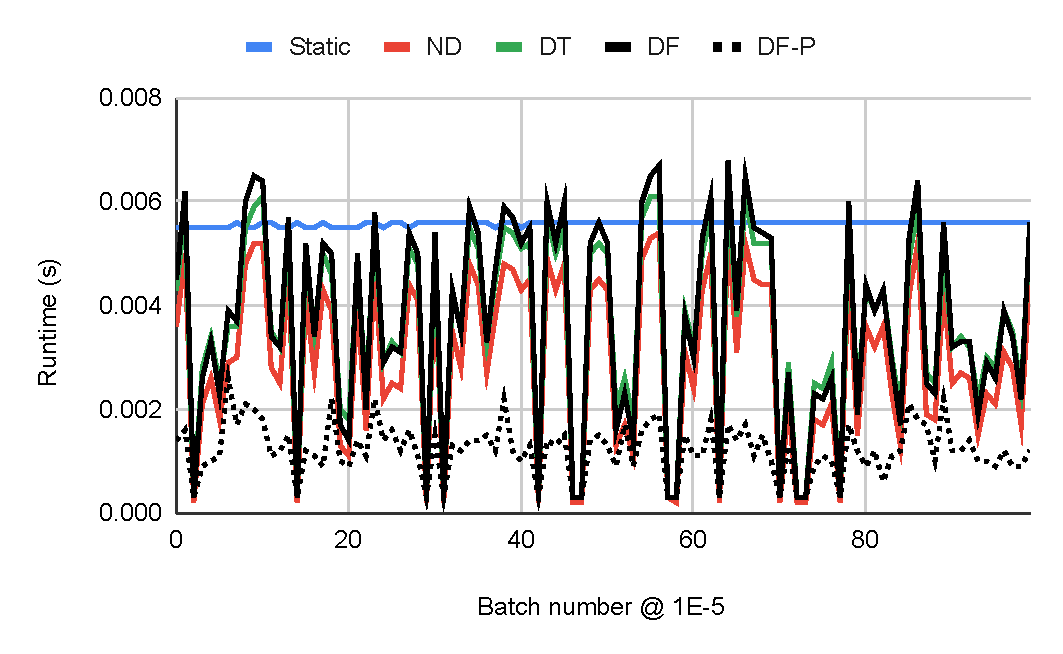
\includegraphics[width=0.48\linewidth]{out/temporal-sx-mathoverflow-runtime5.pdf}
  }
  \subfigure[Error in ranks obtained on consecutive batch updates of size $10^{-5}|E_T|$]{
    \label{fig:temporal-sx-mathoverflow--error5}
    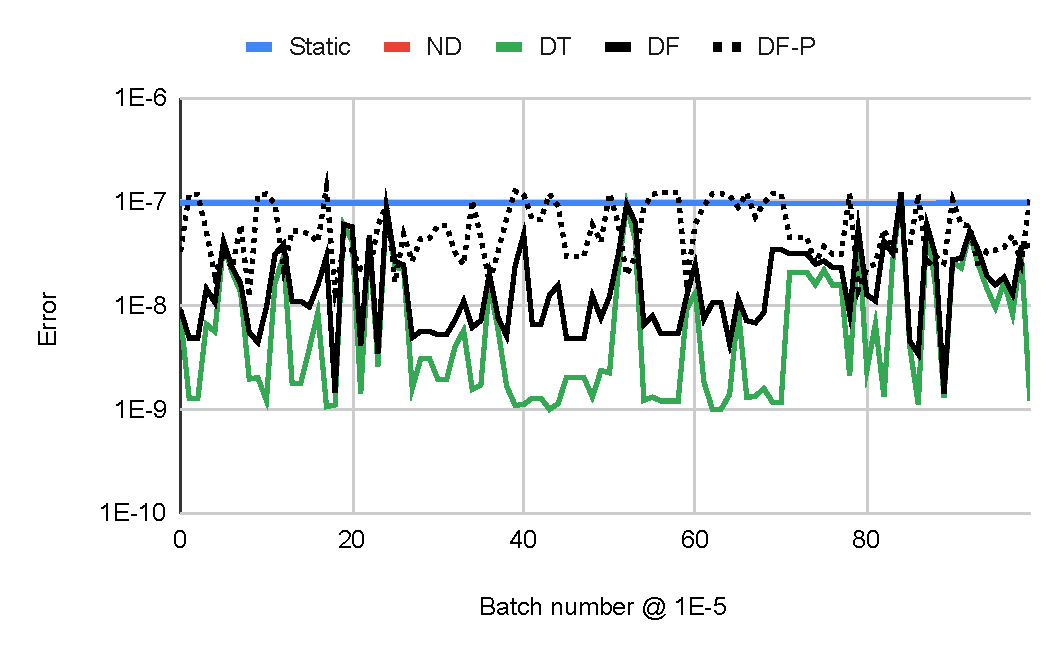
\includegraphics[width=0.48\linewidth]{out/temporal-sx-mathoverflow-error5.pdf}
  } \\[2ex]
  \subfigure[Runtime on consecutive batch updates of size $10^{-4}|E_T|$]{
    \label{fig:temporal-sx-mathoverflow--runtime4}
    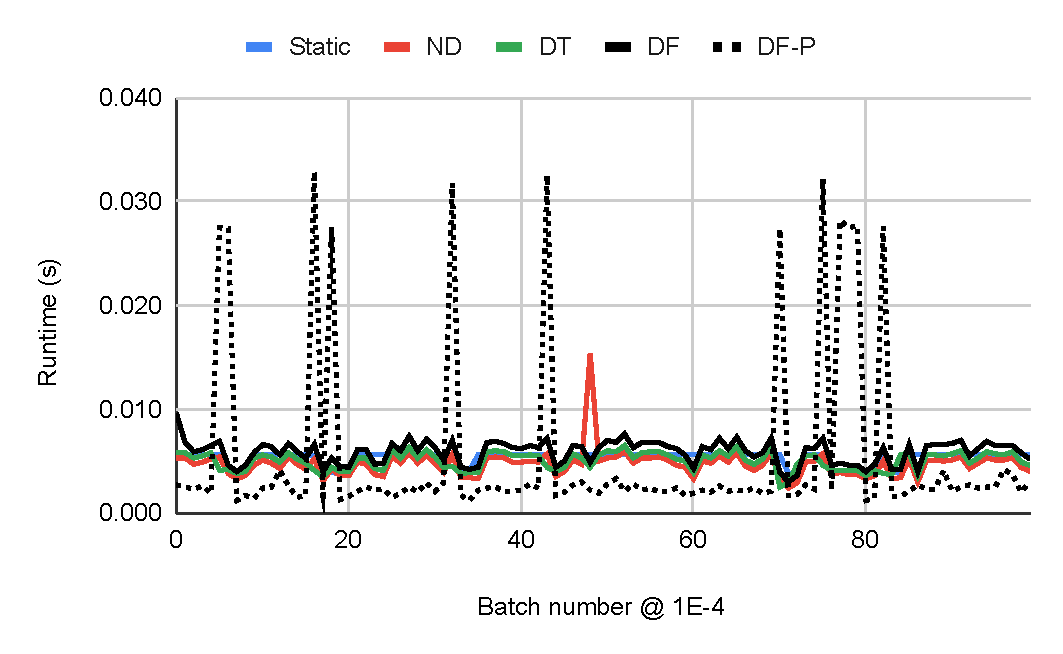
\includegraphics[width=0.48\linewidth]{out/temporal-sx-mathoverflow-runtime4.pdf}
  }
  \subfigure[Error in ranks obtained on consecutive batch updates of size $10^{-4}|E_T|$]{
    \label{fig:temporal-sx-mathoverflow--error4}
    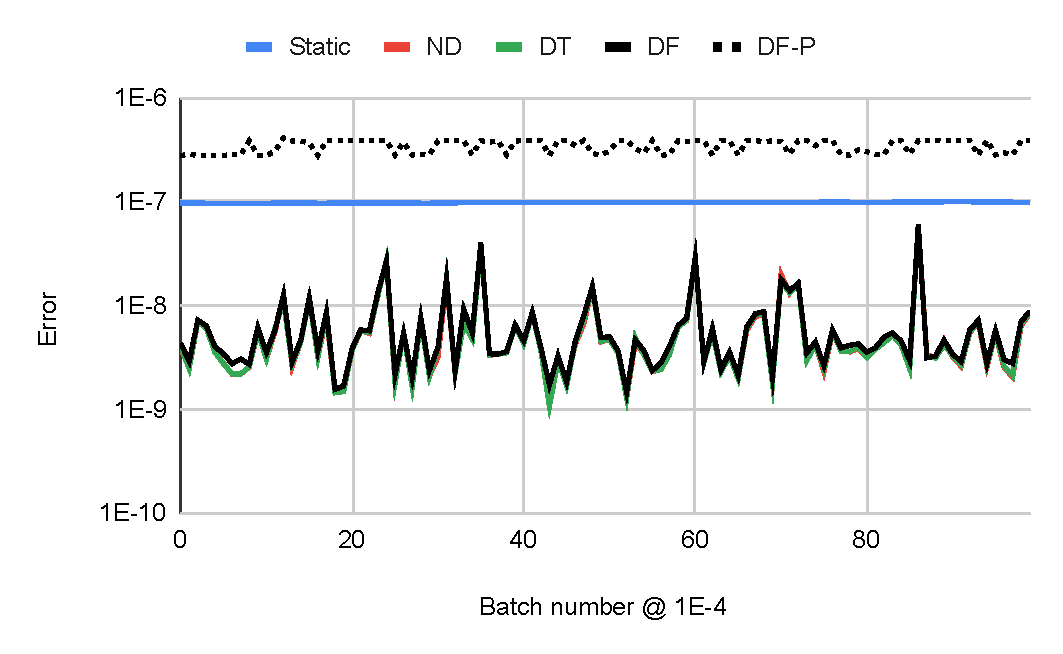
\includegraphics[width=0.48\linewidth]{out/temporal-sx-mathoverflow-error4.pdf}
  } \\[2ex]
  \subfigure[Runtime on consecutive batch updates of size $10^{-3}|E_T|$]{
    \label{fig:temporal-sx-mathoverflow--runtime3}
    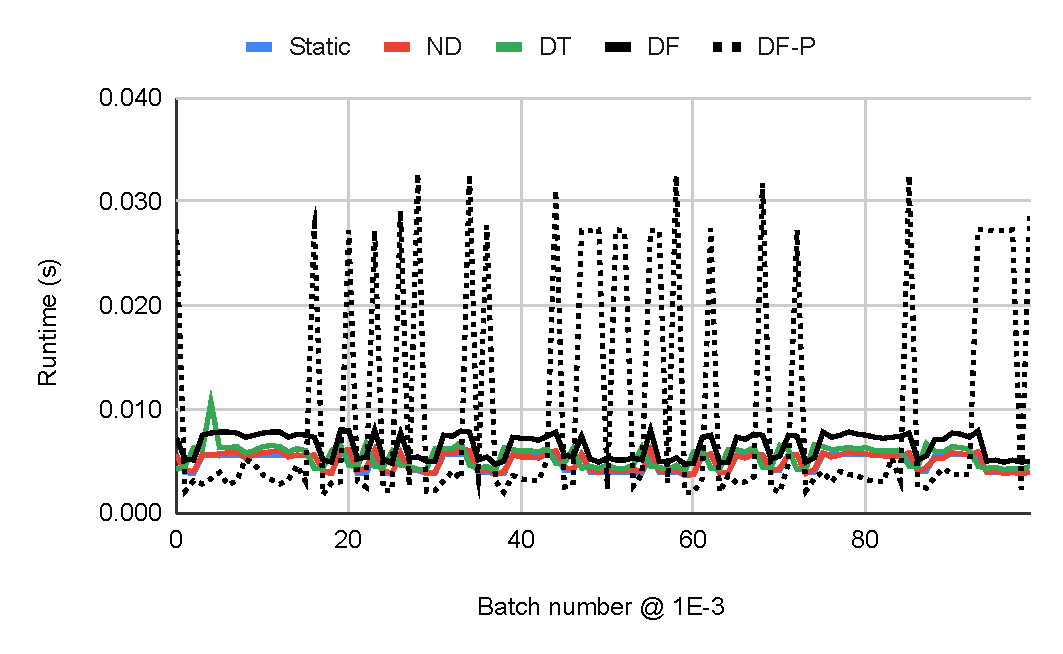
\includegraphics[width=0.48\linewidth]{out/temporal-sx-mathoverflow-runtime3.pdf}
  }
  \subfigure[Error in ranks obtained on consecutive batch updates of size $10^{-3}|E_T|$]{
    \label{fig:temporal-sx-mathoverflow--error3}
    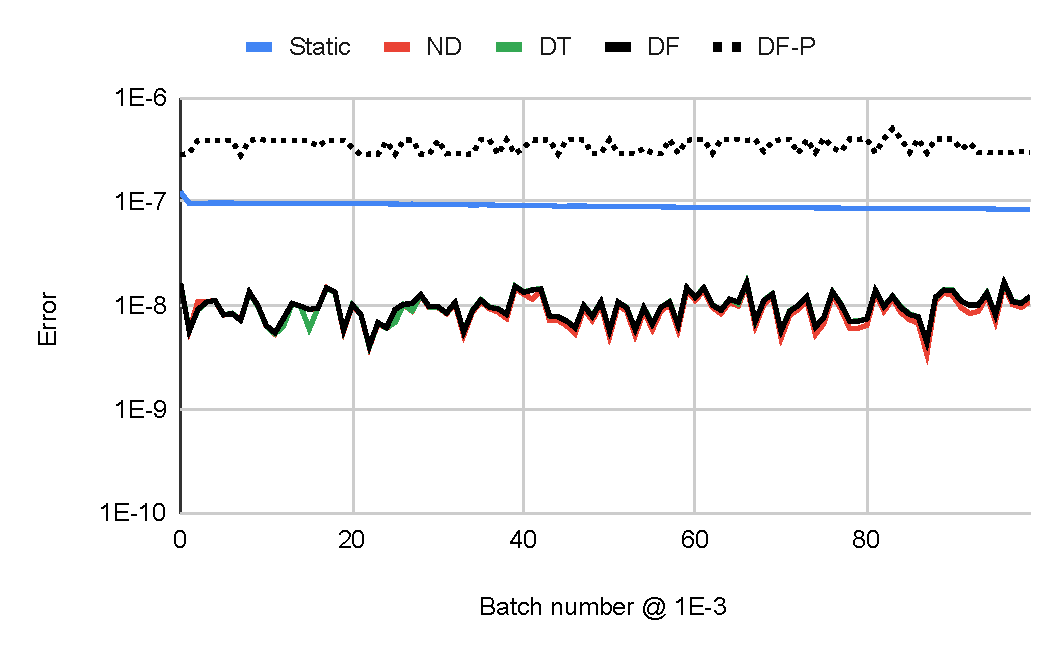
\includegraphics[width=0.48\linewidth]{out/temporal-sx-mathoverflow-error3.pdf}
  } \\[-2ex]
  \caption{Runtime and Error in ranks obtained with \textit{Static}, \textit{Naive-dynamic (ND)}, \textit{Dynamic Traversal (DT)}, our improved \textit{Dynamic Frontier (DF)}, and our improved \textit{Dynamic Frontier with Pruning (DF-P)} PageRank on the \textit{sx-mathoverflow} dynamic graph. The size of batch updates range from $10^{-5}|E_T|$ to $10^{-3}|E_T|$. The rank error with each approach is measured relative to ranks obtained with a reference Static PageRank run, as detailed in Section \ref{sec:measurement}. \su{TOWR}}
  \label{fig:temporal-sx-mathoverflow}
\end{figure*}

\begin{figure*}[!hbt]
  \centering
  \subfigure[Runtime on consecutive batch updates of size $10^{-5}|E_T|$]{
    \label{fig:temporal-sx-askubuntu--runtime5}
    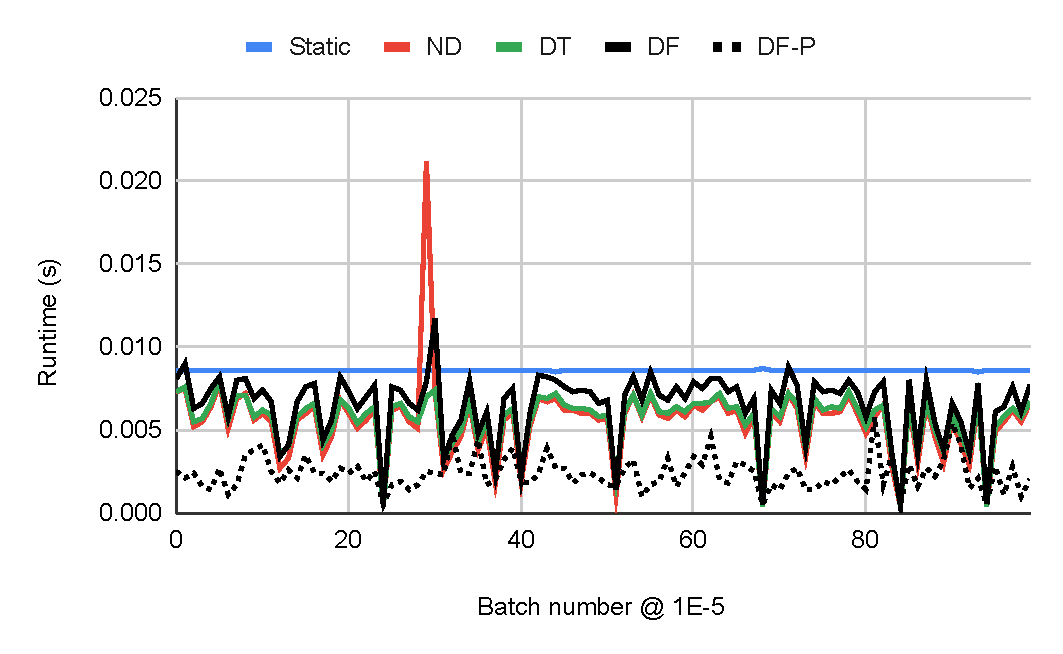
\includegraphics[width=0.48\linewidth]{out/temporal-sx-askubuntu-runtime5.pdf}
  }
  \subfigure[Error in ranks obtained on consecutive batch updates of size $10^{-5}|E_T|$]{
    \label{fig:temporal-sx-askubuntu--error5}
    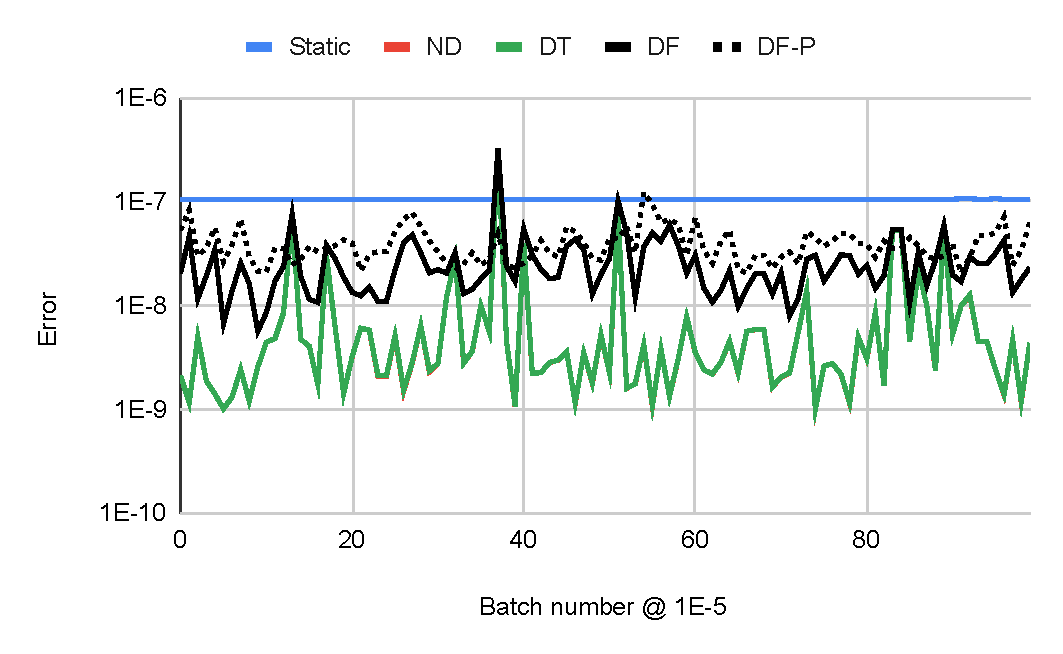
\includegraphics[width=0.48\linewidth]{out/temporal-sx-askubuntu-error5.pdf}
  } \\[2ex]
  \subfigure[Runtime on consecutive batch updates of size $10^{-4}|E_T|$]{
    \label{fig:temporal-sx-askubuntu--runtime4}
    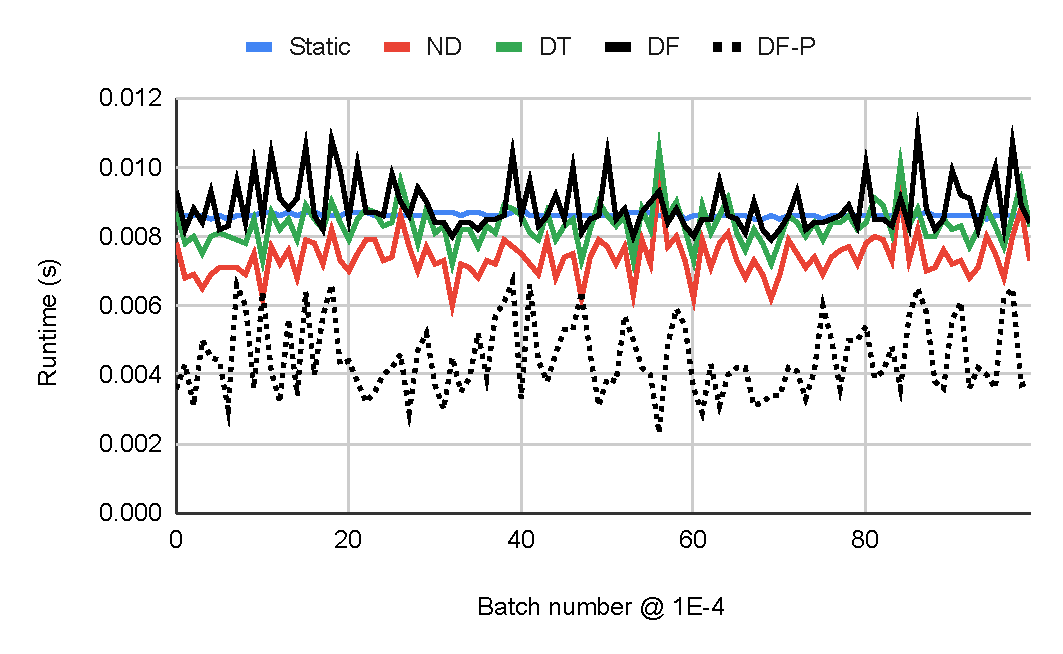
\includegraphics[width=0.48\linewidth]{out/temporal-sx-askubuntu-runtime4.pdf}
  }
  \subfigure[Error in ranks obtained on consecutive batch updates of size $10^{-4}|E_T|$]{
    \label{fig:temporal-sx-askubuntu--error4}
    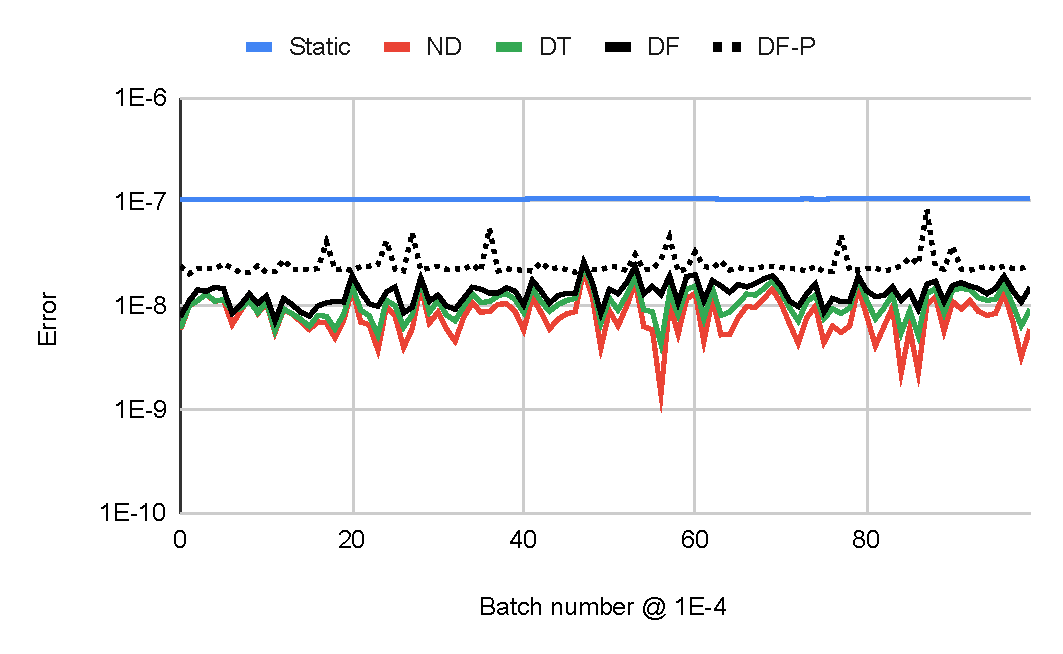
\includegraphics[width=0.48\linewidth]{out/temporal-sx-askubuntu-error4.pdf}
  } \\[2ex]
  \subfigure[Runtime on consecutive batch updates of size $10^{-3}|E_T|$]{
    \label{fig:temporal-sx-askubuntu--runtime3}
    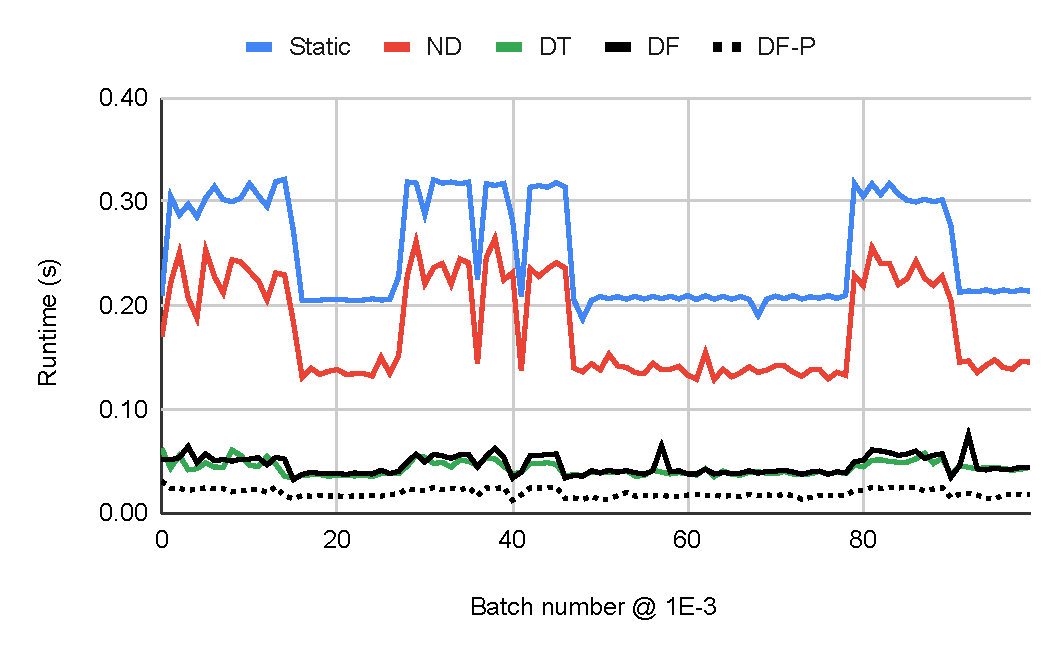
\includegraphics[width=0.48\linewidth]{out/temporal-sx-askubuntu-runtime3.pdf}
  }
  \subfigure[Error in ranks obtained on consecutive batch updates of size $10^{-3}|E_T|$]{
    \label{fig:temporal-sx-askubuntu--error3}
    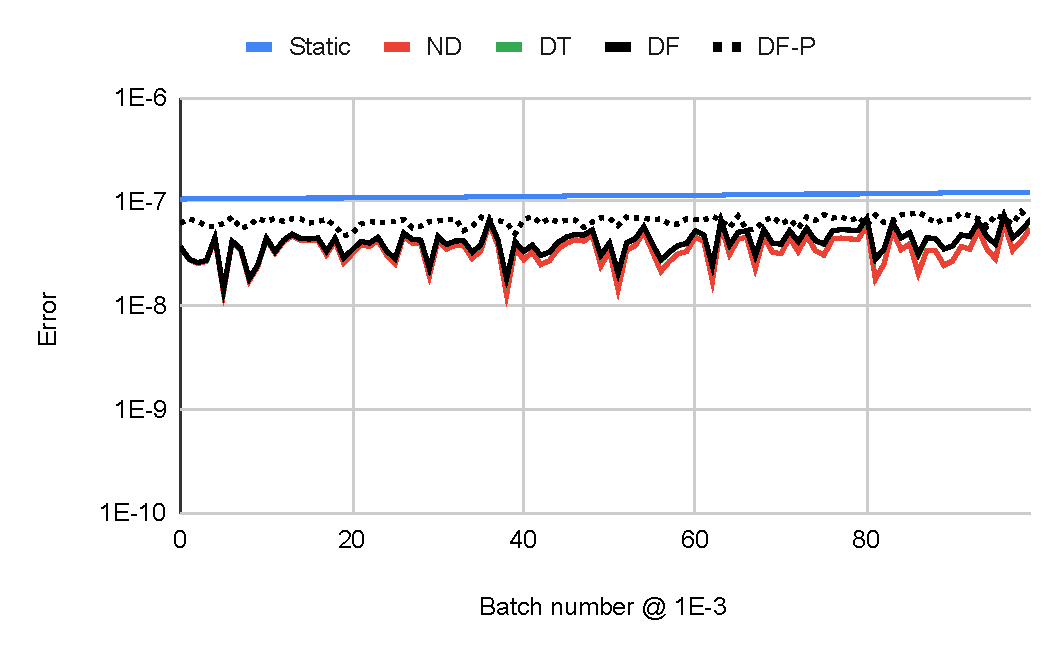
\includegraphics[width=0.48\linewidth]{out/temporal-sx-askubuntu-error3.pdf}
  } \\[-2ex]
  \caption{Runtime and Error in ranks obtained with our GPU implementation of \textit{Static}, \textit{Naive-dynamic (ND)}, \textit{Dynamic Traversal (DT)}, \textit{Dynamic Frontier (DF)}, and \textit{Dynamic Frontier with Pruning (DF-P)} PageRank on the \textit{sx-askubuntu} dynamic graph. The size of batch updates range from $10^{-5}|E_T|$ to $10^{-3}|E_T|$. The rank error with each approach is measured relative to ranks obtained with a reference Static PageRank run, as detailed in Section \ref{sec:measurement}.}
  \label{fig:temporal-sx-askubuntu}
\end{figure*}

\begin{figure*}[!hbt]
  \centering
  \subfigure[Runtime on consecutive batch updates of size $10^{-5}|E_T|$]{
    \label{fig:temporal-sx-superuser--runtime5}
    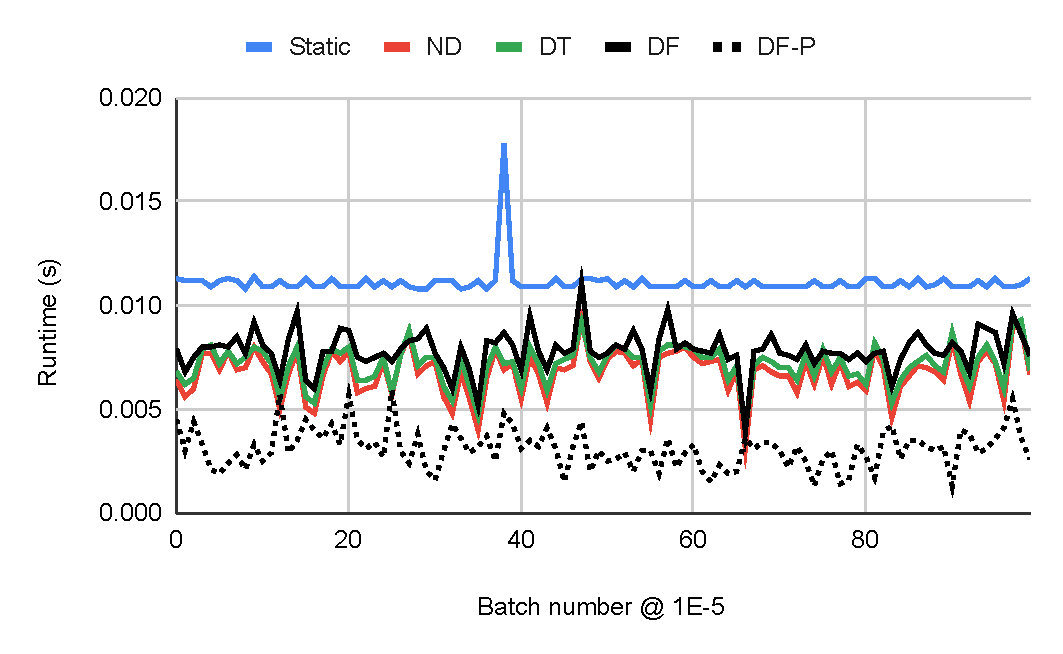
\includegraphics[width=0.48\linewidth]{out/temporal-sx-superuser-runtime5.pdf}
  }
  \subfigure[Error in ranks obtained on consecutive batch updates of size $10^{-5}|E_T|$]{
    \label{fig:temporal-sx-superuser--error5}
    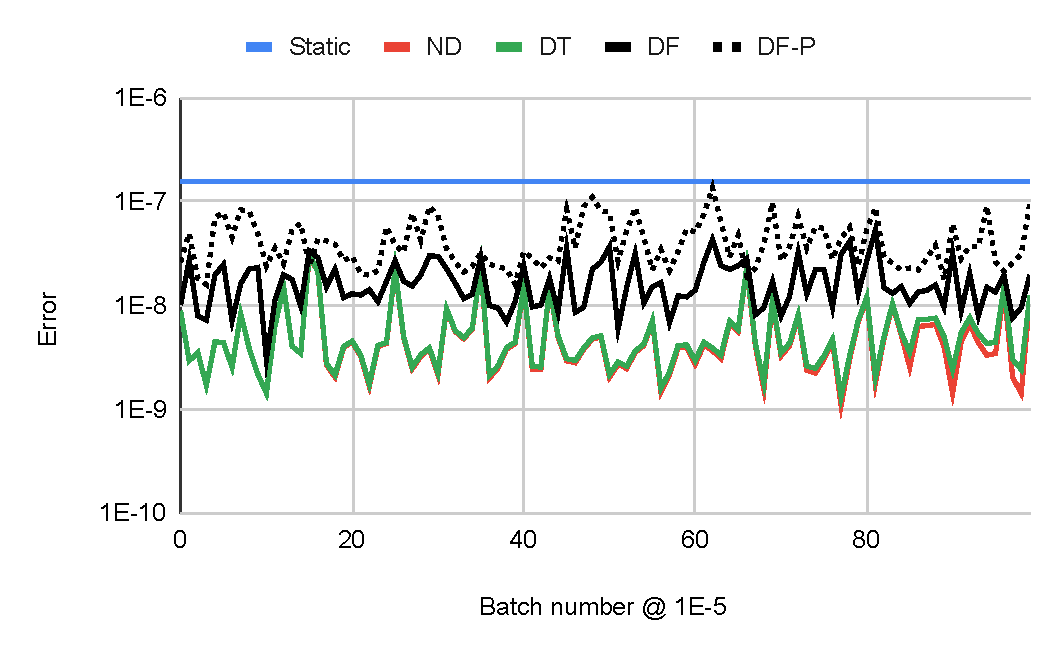
\includegraphics[width=0.48\linewidth]{out/temporal-sx-superuser-error5.pdf}
  } \\[2ex]
  \subfigure[Runtime on consecutive batch updates of size $10^{-4}|E_T|$]{
    \label{fig:temporal-sx-superuser--runtime4}
    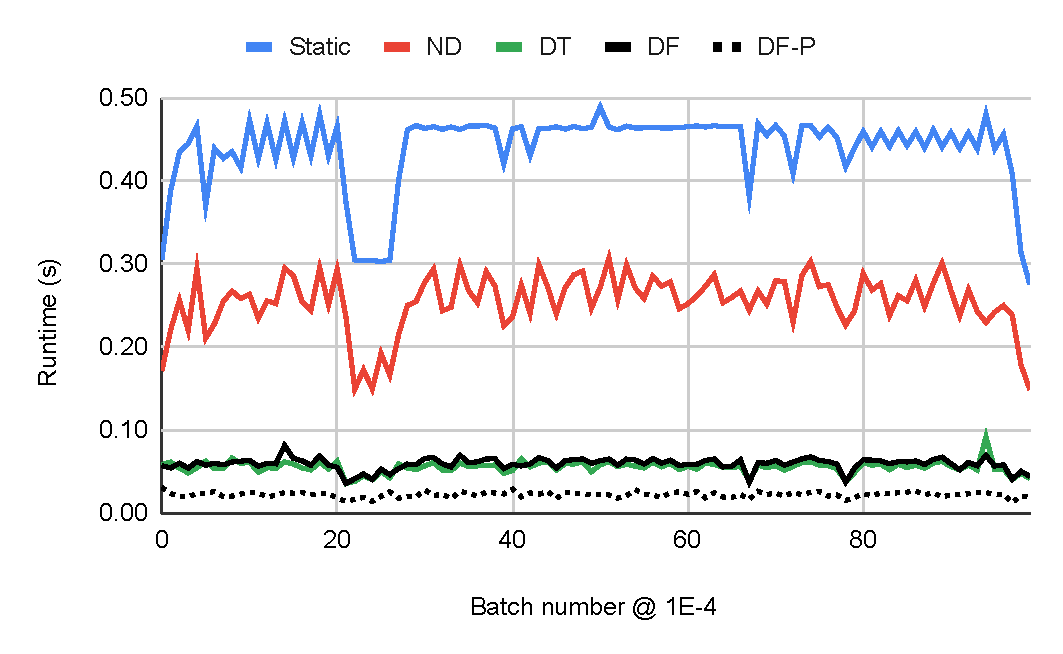
\includegraphics[width=0.48\linewidth]{out/temporal-sx-superuser-runtime4.pdf}
  }
  \subfigure[Error in ranks obtained on consecutive batch updates of size $10^{-4}|E_T|$]{
    \label{fig:temporal-sx-superuser--error4}
    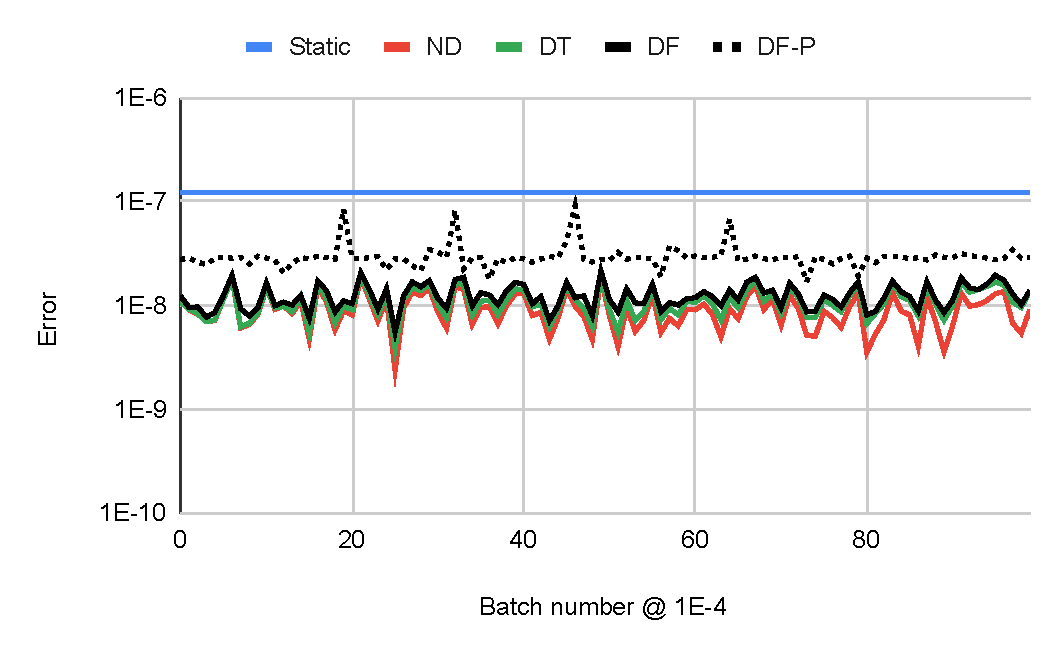
\includegraphics[width=0.48\linewidth]{out/temporal-sx-superuser-error4.pdf}
  } \\[2ex]
  \subfigure[Runtime on consecutive batch updates of size $10^{-3}|E_T|$]{
    \label{fig:temporal-sx-superuser--runtime3}
    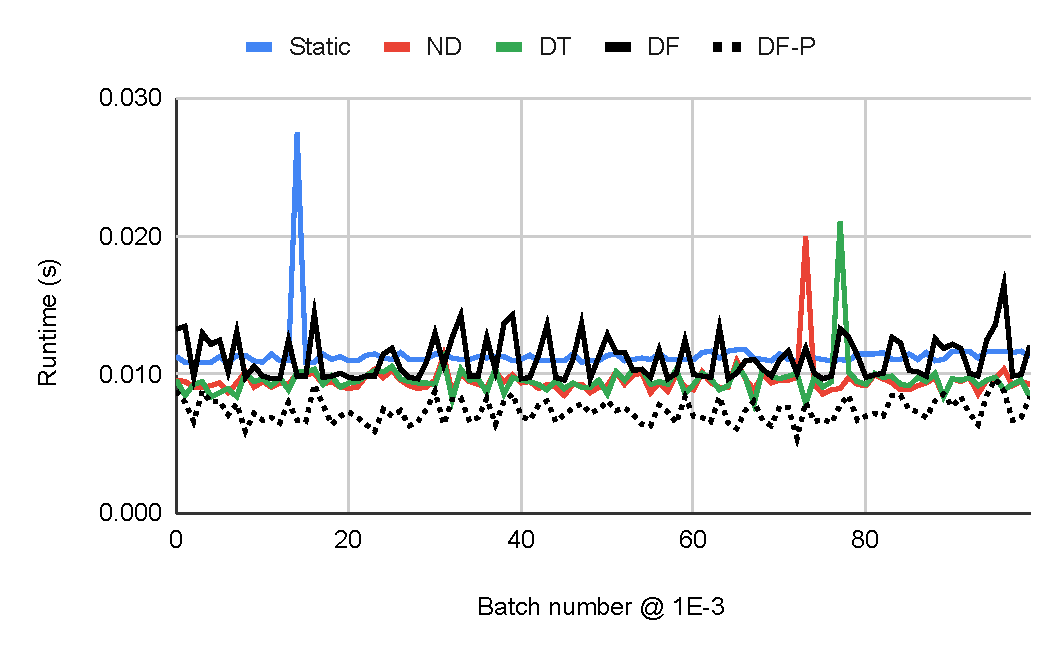
\includegraphics[width=0.48\linewidth]{out/temporal-sx-superuser-runtime3.pdf}
  }
  \subfigure[Error in ranks obtained on consecutive batch updates of size $10^{-3}|E_T|$]{
    \label{fig:temporal-sx-superuser--error3}
    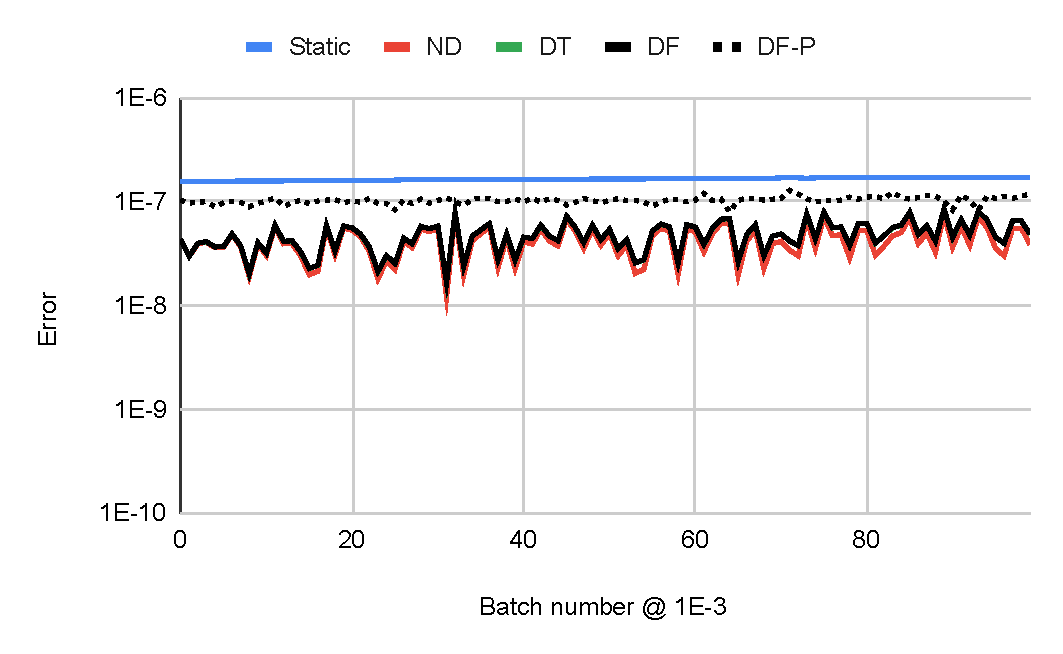
\includegraphics[width=0.48\linewidth]{out/temporal-sx-superuser-error3.pdf}
  } \\[-2ex]
  \caption{Runtime and Error in ranks obtained with \textit{Static}, \textit{Naive-dynamic (ND)}, \textit{Dynamic Traversal (DT)}, our improved \textit{Dynamic Frontier (DF)}, and our improved \textit{Dynamic Frontier with Pruning (DF-P)} PageRank on the \textit{sx-superuser} dynamic graph. The size of batch updates range from $10^{-5}|E_T|$ to $10^{-3}|E_T|$. The rank error with each approach is measured relative to ranks obtained with a reference Static PageRank run, as detailed in Section \ref{sec:measurement}.}
  \label{fig:temporal-sx-superuser}
\end{figure*}

\begin{figure*}[!hbt]
  \centering
  \subfigure[Runtime on consecutive batch updates of size $10^{-5}|E_T|$]{
    \label{fig:temporal-wiki-talk-temporal--runtime5}
    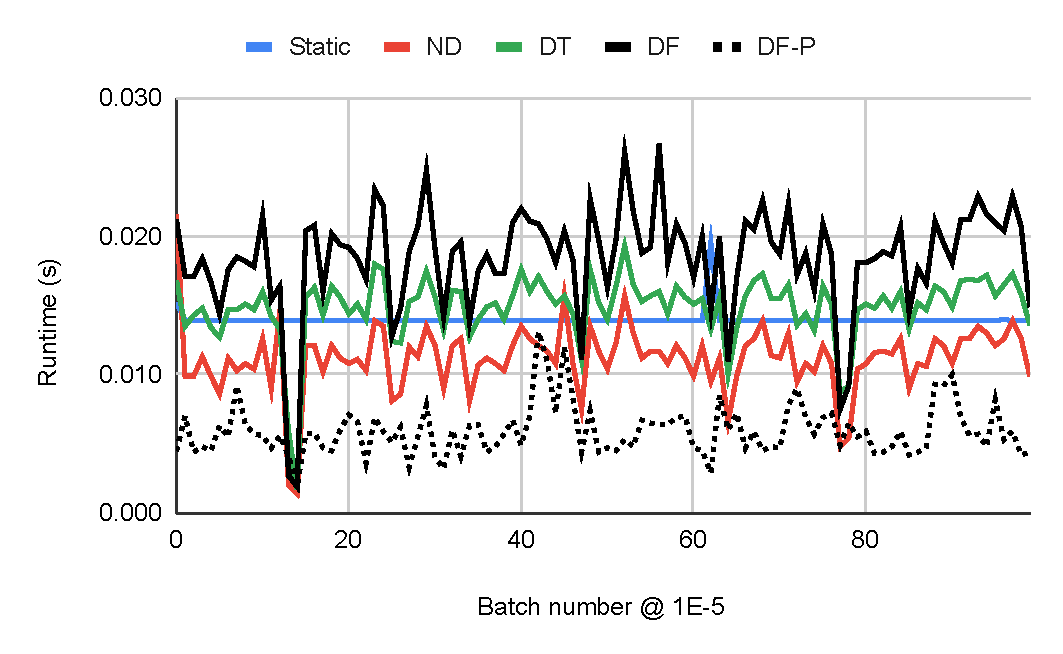
\includegraphics[width=0.48\linewidth]{out/temporal-wiki-talk-temporal-runtime5.pdf}
  }
  \subfigure[Error in ranks obtained on consecutive batch updates of size $10^{-5}|E_T|$]{
    \label{fig:temporal-wiki-talk-temporal--error5}
    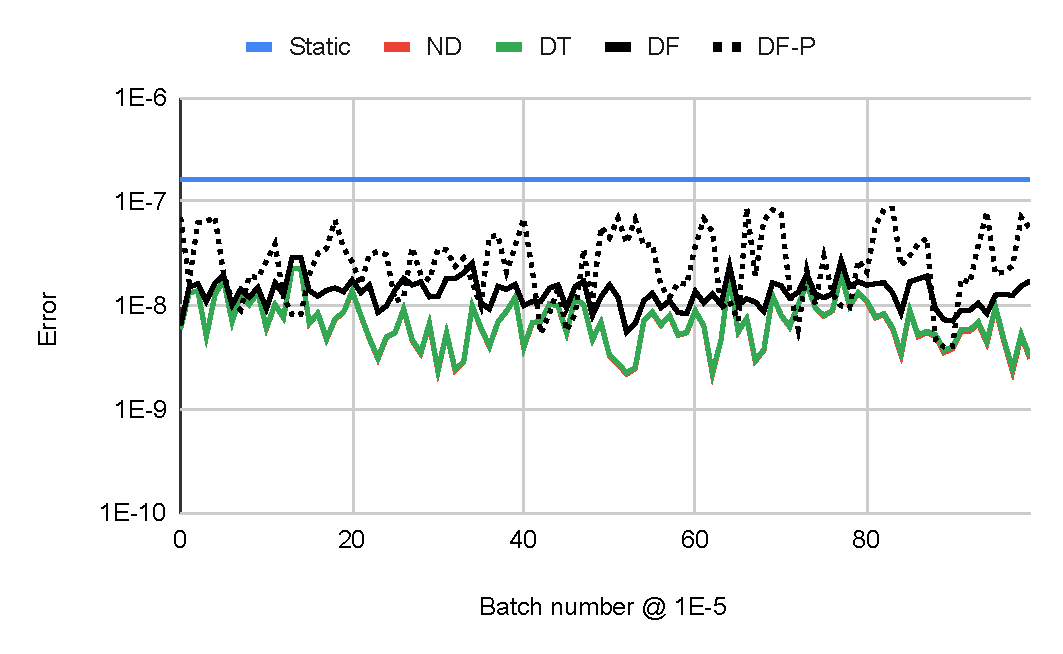
\includegraphics[width=0.48\linewidth]{out/temporal-wiki-talk-temporal-error5.pdf}
  } \\[2ex]
  \subfigure[Runtime on consecutive batch updates of size $10^{-4}|E_T|$]{
    \label{fig:temporal-wiki-talk-temporal--runtime4}
    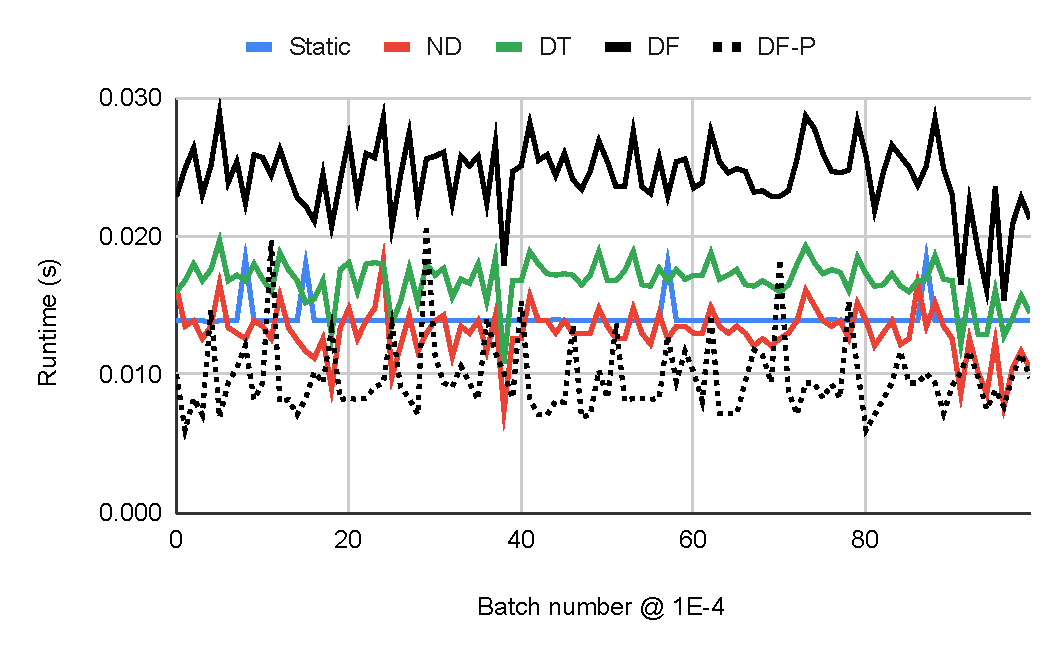
\includegraphics[width=0.48\linewidth]{out/temporal-wiki-talk-temporal-runtime4.pdf}
  }
  \subfigure[Error in ranks obtained on consecutive batch updates of size $10^{-4}|E_T|$]{
    \label{fig:temporal-wiki-talk-temporal--error4}
    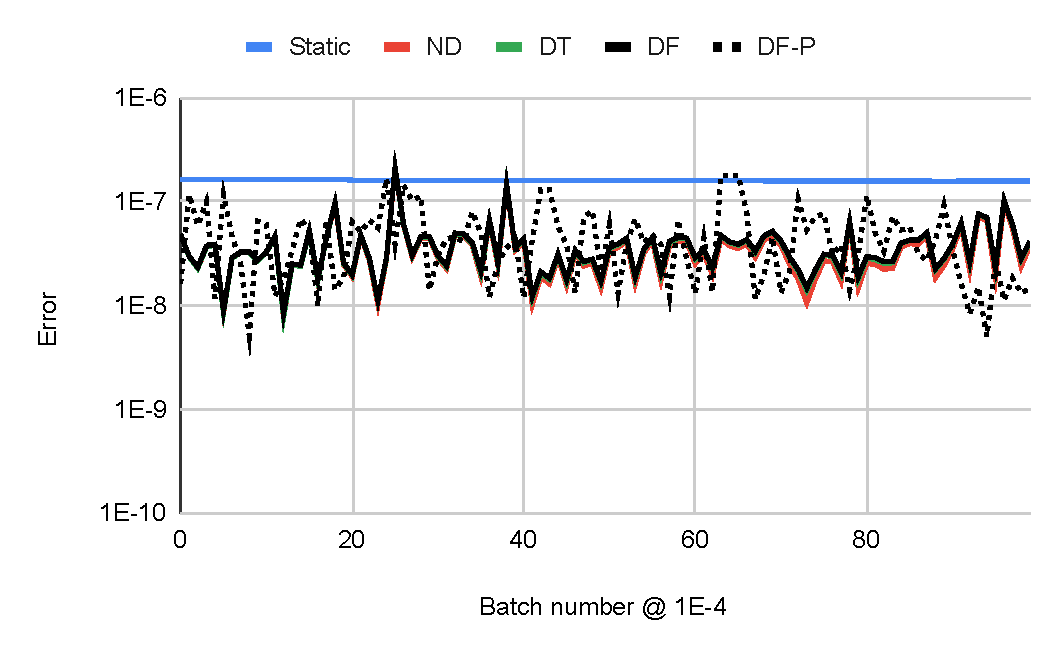
\includegraphics[width=0.48\linewidth]{out/temporal-wiki-talk-temporal-error4.pdf}
  } \\[2ex]
  \subfigure[Runtime on consecutive batch updates of size $10^{-3}|E_T|$]{
    \label{fig:temporal-wiki-talk-temporal--runtime3}
    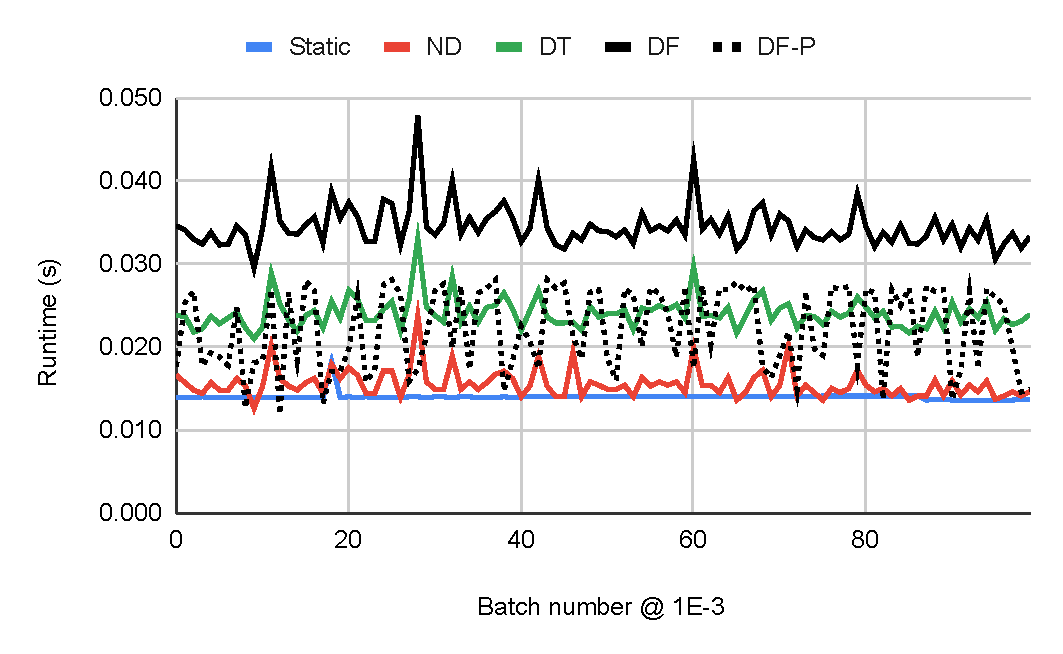
\includegraphics[width=0.48\linewidth]{out/temporal-wiki-talk-temporal-runtime3.pdf}
  }
  \subfigure[Error in ranks obtained on consecutive batch updates of size $10^{-3}|E_T|$]{
    \label{fig:temporal-wiki-talk-temporal--error3}
    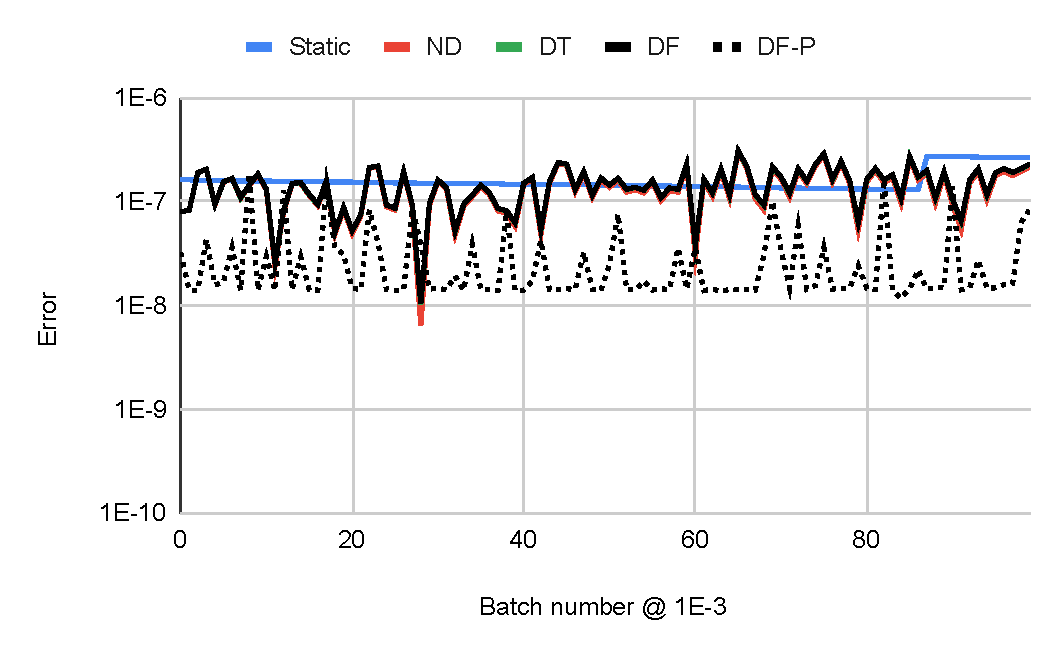
\includegraphics[width=0.48\linewidth]{out/temporal-wiki-talk-temporal-error3.pdf}
  } \\[-2ex]
  \caption{Runtime and Error in ranks obtained with our GPU implementation of \textit{Static}, \textit{Naive-dynamic (ND)}, \textit{Dynamic Traversal (DT)}, \textit{Dynamic Frontier (DF)}, and \textit{Dynamic Frontier with Pruning (DF-P)} PageRank on the \textit{wiki-talk-temporal} dynamic graph. The size of batch updates range from $10^{-5}|E_T|$ to $10^{-3}|E_T|$. The rank error with each approach is measured relative to ranks obtained with a reference Static PageRank run, as detailed in Section \ref{sec:measurement}.}
  \label{fig:temporal-wiki-talk-temporal}
\end{figure*}

\begin{figure*}[!hbt]
  \centering
  \subfigure[Runtime on consecutive batch updates of size $10^{-5}|E_T|$]{
    \label{fig:temporal-sx-stackoverflow--runtime5}
    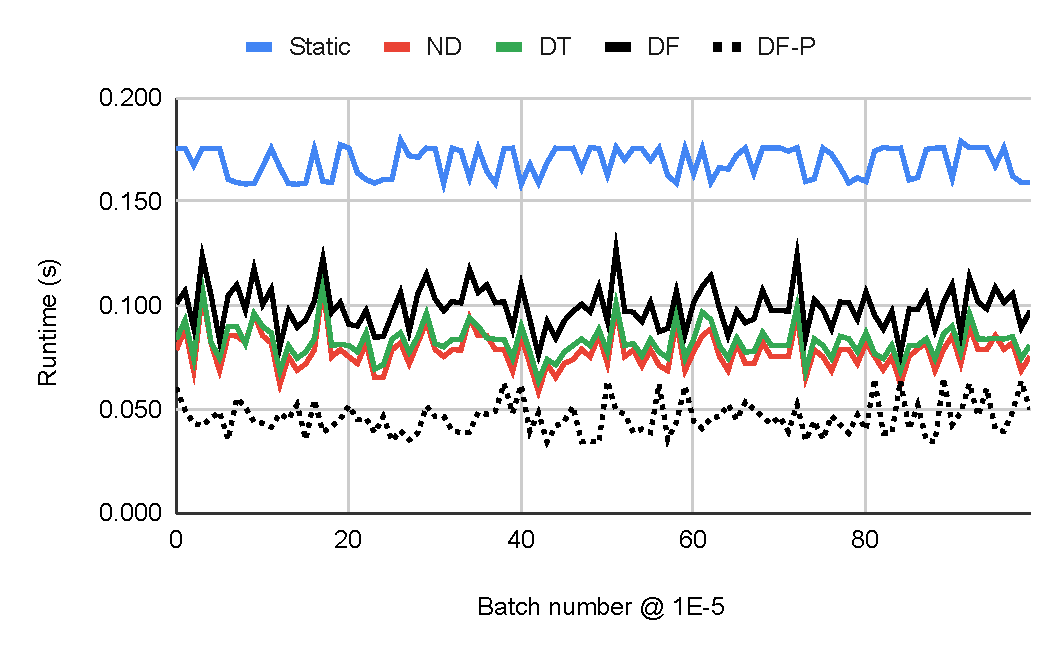
\includegraphics[width=0.48\linewidth]{out/temporal-sx-stackoverflow-runtime5.pdf}
  }
  \subfigure[Error in ranks obtained on consecutive batch updates of size $10^{-5}|E_T|$]{
    \label{fig:temporal-sx-stackoverflow--error5}
    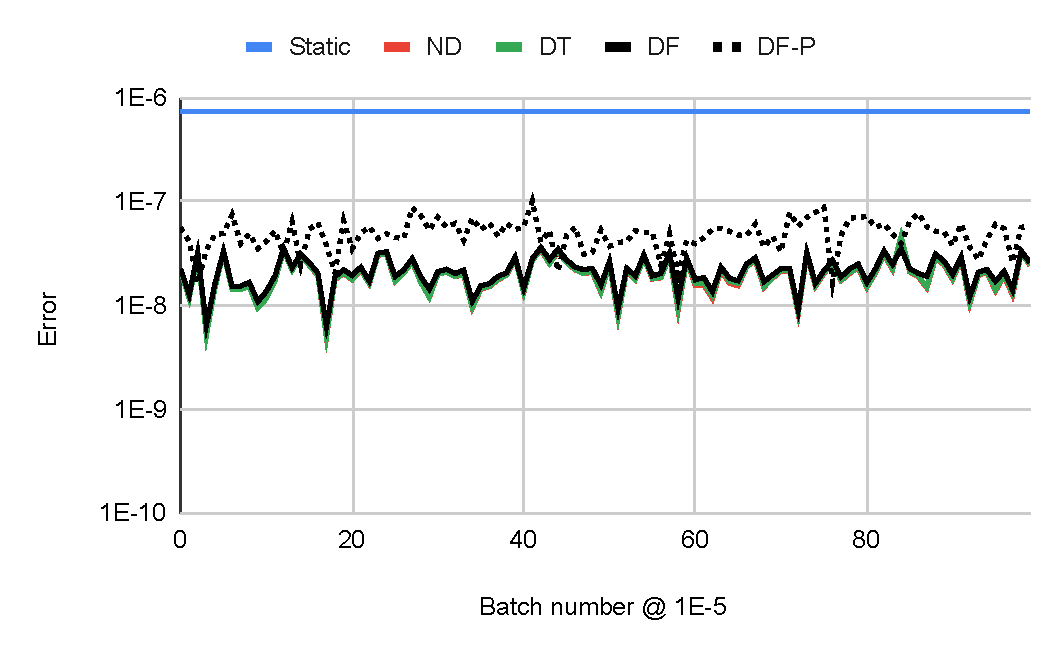
\includegraphics[width=0.48\linewidth]{out/temporal-sx-stackoverflow-error5.pdf}
  } \\[2ex]
  \subfigure[Runtime on consecutive batch updates of size $10^{-4}|E_T|$]{
    \label{fig:temporal-sx-stackoverflow--runtime4}
    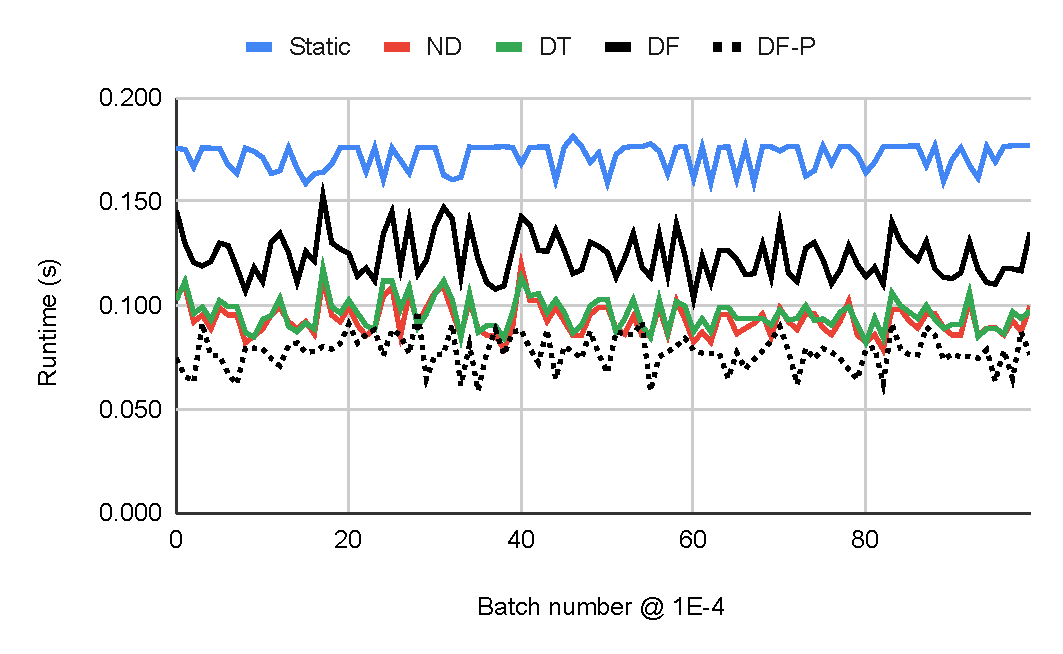
\includegraphics[width=0.48\linewidth]{out/temporal-sx-stackoverflow-runtime4.pdf}
  }
  \subfigure[Error in ranks obtained on consecutive batch updates of size $10^{-4}|E_T|$]{
    \label{fig:temporal-sx-stackoverflow--error4}
    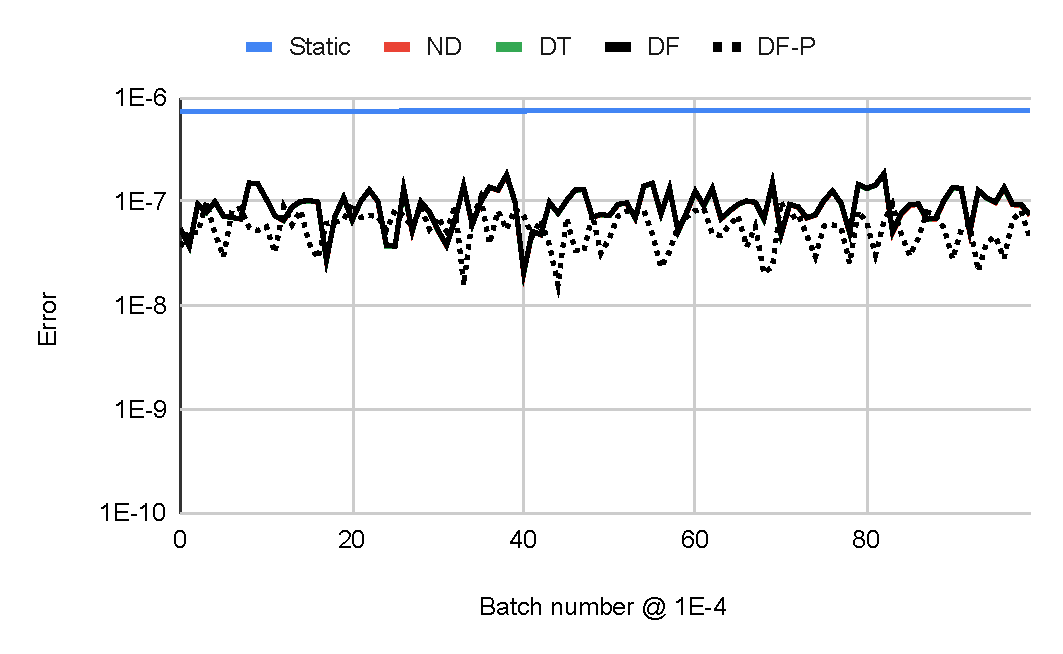
\includegraphics[width=0.48\linewidth]{out/temporal-sx-stackoverflow-error4.pdf}
  } \\[2ex]
  \subfigure[Runtime on consecutive batch updates of size $10^{-3}|E_T|$]{
    \label{fig:temporal-sx-stackoverflow--runtime3}
    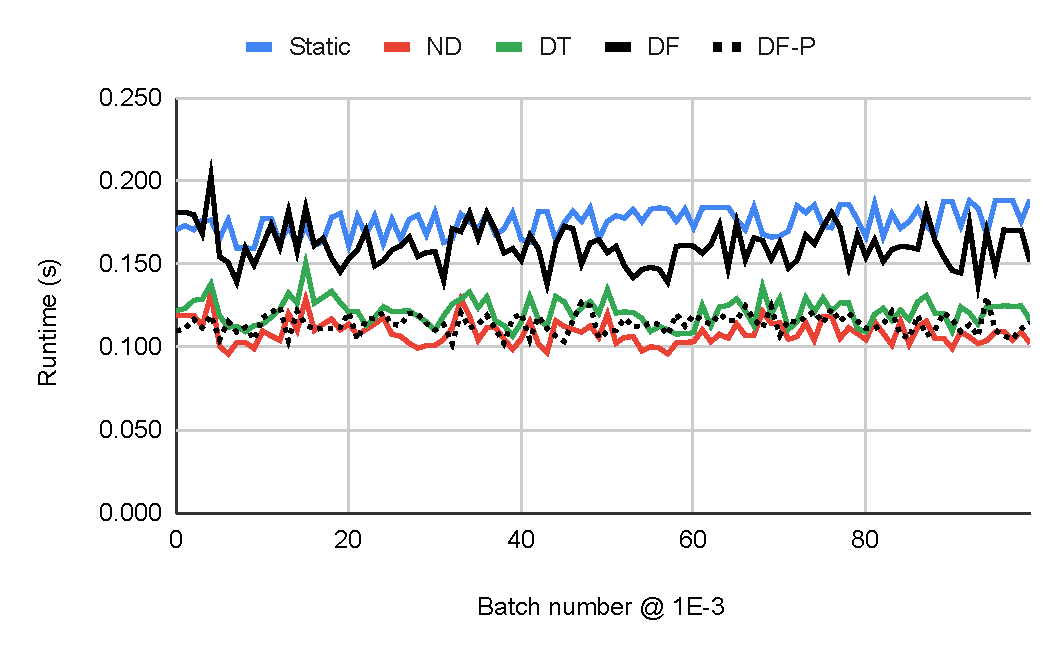
\includegraphics[width=0.48\linewidth]{out/temporal-sx-stackoverflow-runtime3.pdf}
  }
  \subfigure[Error in ranks obtained on consecutive batch updates of size $10^{-3}|E_T|$]{
    \label{fig:temporal-sx-stackoverflow--error3}
    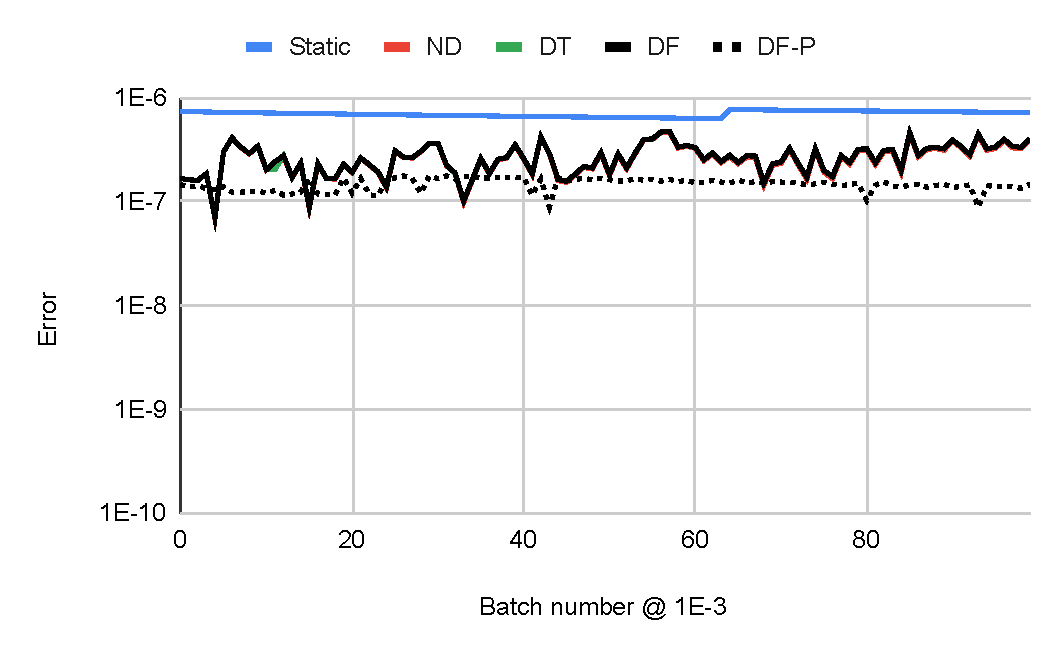
\includegraphics[width=0.48\linewidth]{out/temporal-sx-stackoverflow-error3.pdf}
  } \\[-2ex]
  \caption{Runtime and Error in ranks obtained with \textit{Static}, \textit{Naive-dynamic (ND)}, \textit{Dynamic Traversal (DT)}, our improved \textit{Dynamic Frontier (DF)}, and our improved \textit{Dynamic Frontier with Pruning (DF-P)} PageRank on the \textit{sx-stackoverflow} dynamic graph. The size of batch updates range from $10^{-5}|E_T|$ to $10^{-3}|E_T|$. The rank error with each approach is measured relative to ranks obtained with a reference Static PageRank run, as detailed in Section \ref{sec:measurement}. \su{TOWR}}
  \label{fig:temporal-sx-stackoverflow}
\end{figure*}


\clearpage

\section{Appendix}



\subsection{Updating ranks of vertices in parallel}
\label{sec:update}

Algorithm \ref{alg:update} provides a psuedocode for updating the ranks of vertices in parallel. Here, the function \texttt{updateRanks()} takes as input the set of affected vertices $\delta_V$, affected neighbor vertices $\delta_N$, the previous and current rank vectors $R$ and $R_{new}$, respectively, the current input graph $G^t$, partitioned vertex IDs $P'$ (low in-degree vertices come first), and the number of vertices with low in-degree $N'_P$. It also requires parameters such as the damping factor $\alpha$, frontier tolerance $\tau_f$, and prune tolerance $\tau_p$.

The algorithm operates in two phases: a thread-per-vertex kernel (for low degree vertices) and a block-per-vertex kernel (for high degree vertices). In the \textit{thread-per-vertex kernel} (lines \ref{alg:update--thread-begin}-\ref{alg:update--thread-end}), we use each thread to process each low degree vertex in parallel, iterating over the partitioned vertex IDs ($P'$). For each vertex $v$, if it's not marked as affected, we skip it (line \ref{alg:update--affected}). Otherwise, we compute the new rank $r$ based on the incoming edges and ranks of neighboring vertices (lines \ref{alg:update--rank-begin}-\ref{alg:update--rank-end}). Depending on whether DF or DF-P PageRank is selected, we compute ranks using either Equation \ref{eq:pr} or \ref{eq:pr-prune}, respectively. Next, we compute the change in rank $\Delta r$ of the current vertex $v$ from its previous iteration (line \ref{alg:update--change}). If the relative change in rank of $v$, i.e., $\Delta r / \max(r, R[v])$, is within the prune tolerance $\tau_p$, we perform pruning by marking $v$ and no longer affected. However, if the relative change in rank of $v$ is above the frontier tolerance $\tau_f$, we mark the vertices whose neighbors must be incrementally marked as affected (the incremental marking of affected vertices is performed at a later point of time, using the \texttt{expandAffected()} function (Algorithm \ref{alg:affected}). Finally, we update the rank of vertex $v$ in the $R$ vector. In the \textit{block-per-vertex kernel} (lines \ref{alg:update--block-begin}-\ref{alg:update--block-end}), we use each thread block to process each high degree vertex in parallel, utilizing block-level parallelism. It involves similar operations as the thread-per-vertex kernel, but uses block-reduce operations and shared memory.


\subsection{Parallel vertex partitioning by degree}
\label{sec:partition}

Algorithm \ref{alg:partition} outlines the psuedocode for parallel vertex partitioning by degree. It aims to split the vertices of the input graph $G(V, E)$ into two groups based on their degree: low-degree vertices and high-degree vertices. The algorithm provides partitioned vertex IDs $P$ with low-degree vertices being listed first, along with the number of vertices with low degree $N_P$, as its output.

In the function \texttt{partition()}, we start by initializing an empty buffer $B_k$ and the set of partitioned vertex IDs $P$ (line \ref{alg:partition--initialize}). We then proceed to populate $B_k$ with boolean values indicating whether each vertex has a degree less than or equal to a specified threshold $D_P$ (lines \ref{alg:partition--less-begin}-\ref{alg:partition--less-end}). Afterward, we perform an exclusive prefix sum operation on $B_k$ to determine the number of low-degree vertices $N_P$ (lines \ref{alg:partition--lscan-begin}-\ref{alg:partition--lscan-end}). In the subsequent loop, we assign low-degree vertices to the appropriate positions in the partitioned vertex IDs array $P$ (lines \ref{alg:partition--lpopulate-begin}-\ref{alg:partition--lpopulate-end}). We then repeat a similar process for high-degree vertices. We populate $B_k$ with boolean values indicating whether each vertex has a degree greater than $D_P$ (lines \ref{alg:partition--greater-begin}-\ref{alg:partition--greater-end}), perform another exclusive prefix sum operation on $B_k$ (line \ref{alg:partition--gscan}), and assign high-degree vertices to the appropriate positions in $P$ (lines \ref{alg:partition--gpopulate-begin}-\ref{alg:partition--gpopulate-end}). Finally, we return the partitioned vertex IDs $P$ along with the number of low-degree vertices $N_P$ (line \ref{alg:partition--return}).


\subsection{Parallel marking of affected vertices}
\label{sec:affected}

Algorithm \ref{alg:affected} presents the psuedocode for parallel marking of affected vertices, consisting of two functions: \texttt{initialAffected()} and \texttt{expandAffected()}.

The \texttt{initialAffected()} function performs an initial marking step of DF and DF-P PageRank. It takes as input the current graph snapshot $G^t$ and the sets of edge deletions $\Delta^{t-}$ and insertions $\Delta^{t+}$. Here, we first initialize two arrays, $\delta_V$ and $\delta_N$, which represent whether each vertex and its neighbors are affected, respectively (line \ref{alg:affected--iinitialize}). Next, for each edge deletion in $\Delta^{t-}$, we mark both the source and target vertices as affected (lines \ref{alg:affected--idel-begin}-\ref{alg:affected--idel-end}). Similarly, for each edge insertion in $\Delta^{t+}$, we mark the source vertex as affected (lines \ref{alg:affected--iins-begin}-\ref{alg:affected--iins-end}). Finally, we return $\delta_V$ and $\delta_N$ (line \ref{alg:affected--ireturn}).

The \texttt{expandAffected()} function propagates the affected status to neighboring vertices. It takes as input flags indicating whether each vertex is affected $\delta_V$ or its neighbors are affected $\delta_N$, the current graph snapshot $G^t$, partitioned vertex IDs $P$ with low degree vertices placed first, and the number of vertices with low degree $N_P$. This algorithm also operates in two phases: a thread-per-vertex kernel (for low degree vertices) and a block-per-vertex kernel (for high degree vertices). In the \textit{thread-per-vertex kernel} (lines \ref{alg:affected--ethread-begin}-\ref{alg:affected--ethread-end}), we use each thread to process each low degree vertex in parallel by iterating through the partitioned vertex IDs array $P$. For each vertex $u$ marked as affected in $\delta_N$, we invoke the \texttt{markNeighbors()} function to mark its neighbors as affected in $\delta_V$ (line \ref{alg:affected--etmark}). In the \textit{block-per-vertex kernel} (lines \ref{alg:affected--eblock-begin}-\ref{alg:affected--eblock-end}), we use each thread block to process each vertex in parallel, utilizing block-level parallelism. It involves similar operations as the thread-per-vertex kernel.


\begin{figure*}[!hbt]
  \centering
  \subfigure[Overall Runtime \textbf{(GPU)}]{
    \label{fig:temporal-compare--runtime-overall}
    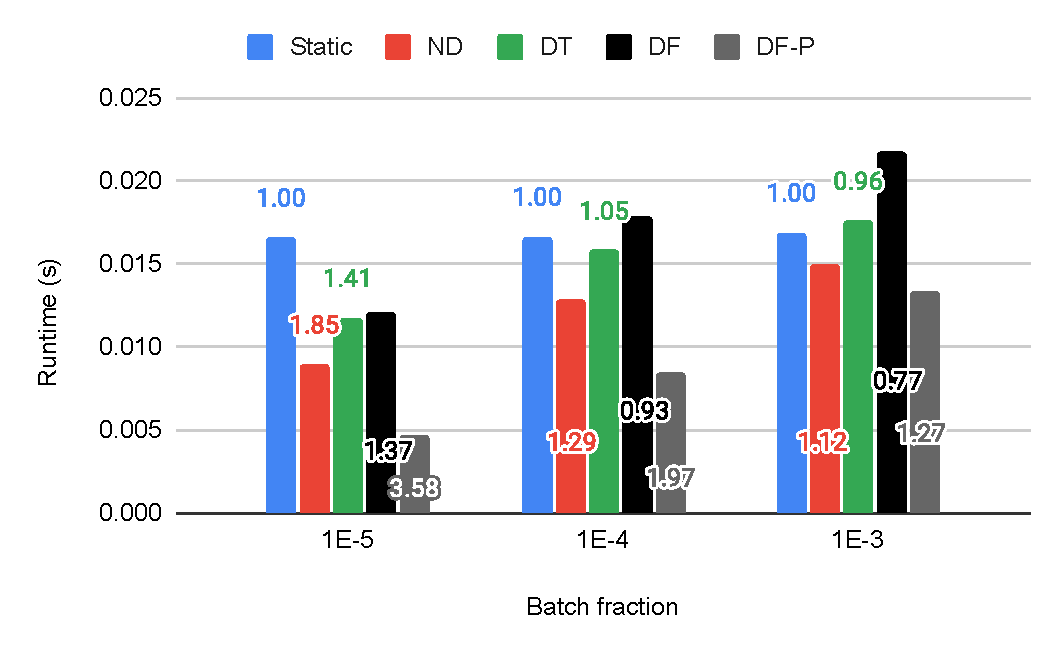
\includegraphics[width=0.48\linewidth]{out/temporal-summary-runtime-overall.pdf}
  }
  \subfigure[Overall Error in ranks obtained \textbf{(GPU)}]{
    \label{fig:temporal-compare--error-overall}
    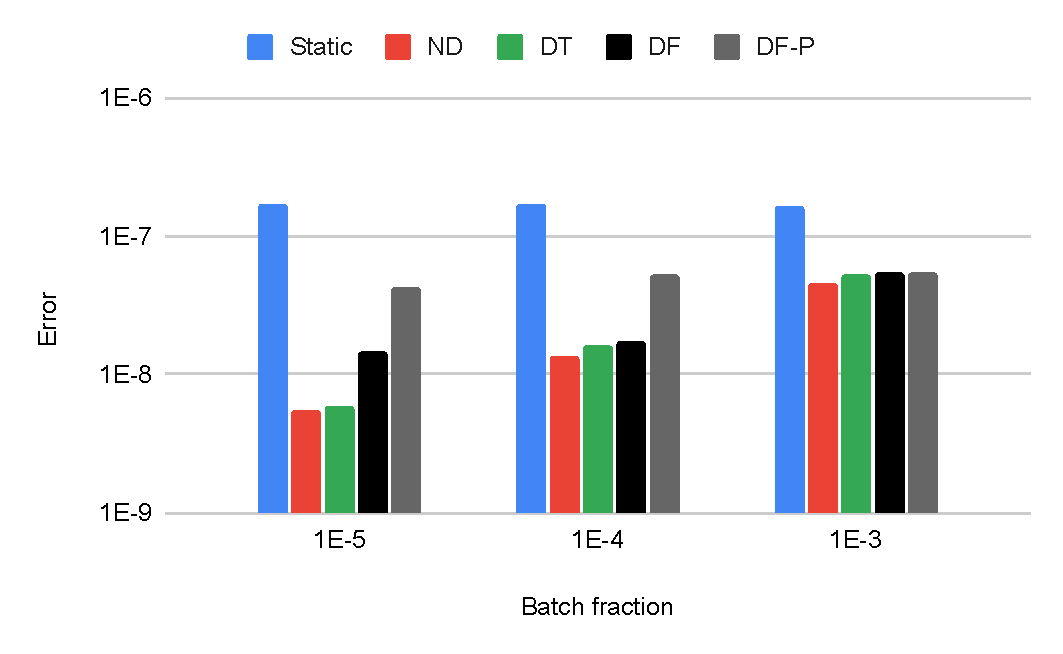
\includegraphics[width=0.48\linewidth]{out/temporal-summary-error-overall.pdf}
  }
  \subfigure[Overall Runtime \textbf{(CPU)}]{
    \label{fig:temporal-compare--runtime-overall-cpu}
    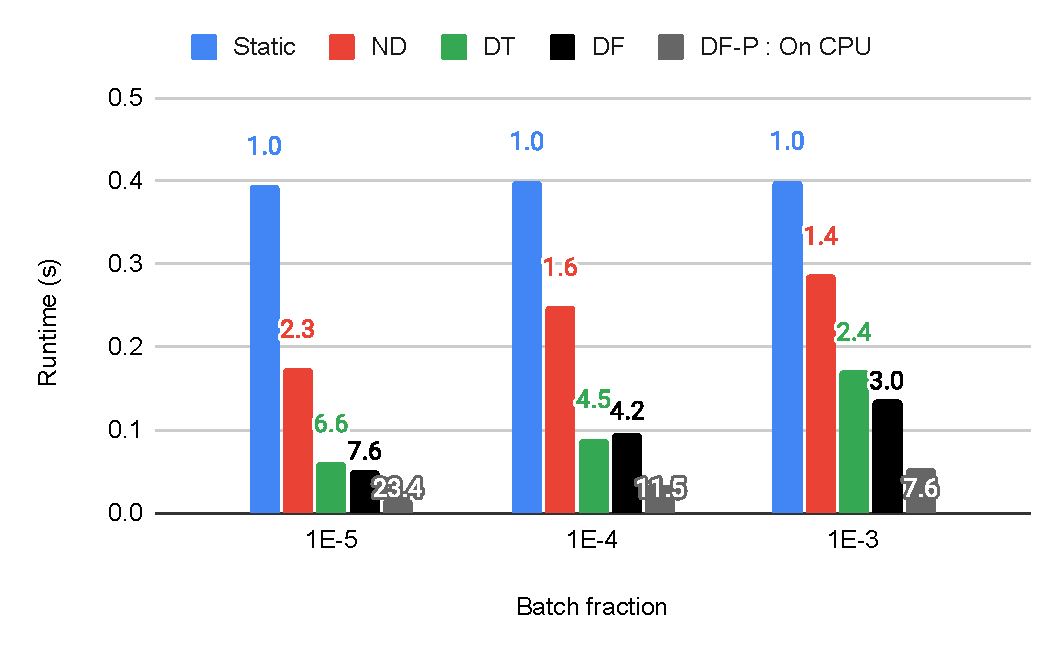
\includegraphics[width=0.48\linewidth]{out/temporal-summary-runtime-overall-cpu.pdf}
  }
  \subfigure[Overall Error in ranks obtained \textbf{(CPU)}]{
    \label{fig:temporal-compare--error-overall-cpu}
    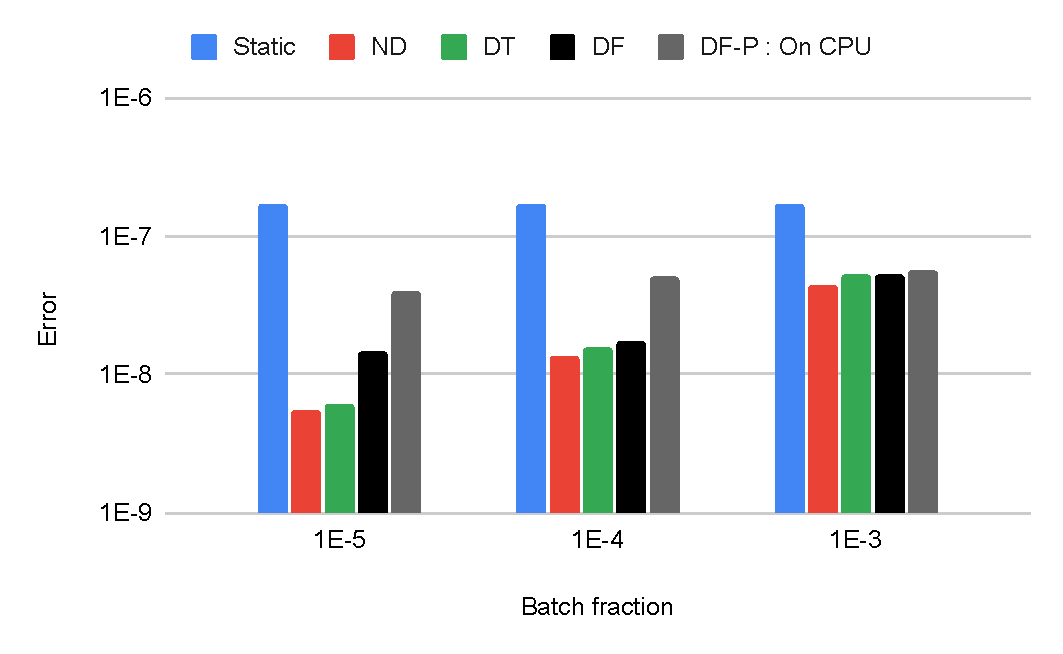
\includegraphics[width=0.48\linewidth]{out/temporal-summary-error-overall-cpu.pdf}
  } \\[-2ex]
  \caption{Mean Runtime and Error in ranks obtained with \textit{Static}, \textit{Naive-dynamic (ND)}, \textit{Dynamic Traversal (DT)}, our improved \textit{Dynamic Frontier (DF)}, and our improved \textit{Dynamic Frontier with Pruning (DF-P)} PageRank on real-world dynamic graphs, with batch updates of size $10^{-5}|E_T|$ to $10^{-3}|E_T|$. Here, (a) and (b) show the overall runtime and error across all temporal graphs, while (c) and (d) show the runtime and rank error for each approach (relative to reference Static PageRank, see Section \ref{sec:measurement}). In (a), the speedup of each approach with respect to Static PageRank is labeled. \su{TOWR}}
  \label{fig:temporal-compare}
\end{figure*}

\begin{figure*}[hbtp]
  \centering
  \subfigure[Overall result \textbf{(GPU)}]{
    \label{fig:8020-runtime-compare--mean}
    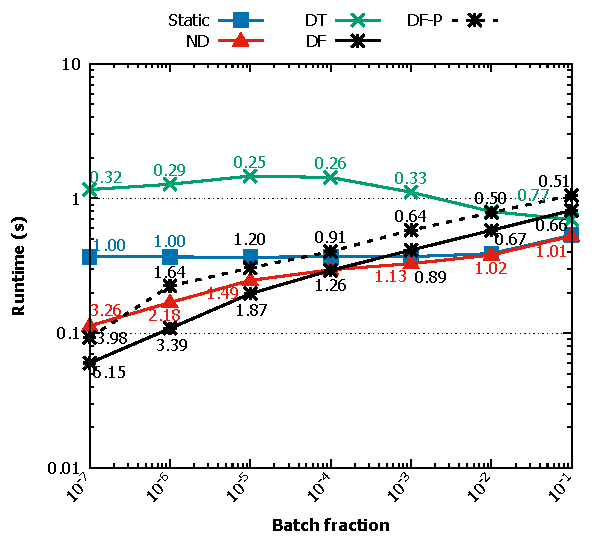
\includegraphics[width=0.38\linewidth]{out/8020-runtime-mean.pdf}
  }
  \subfigure[Results on each graph \textbf{(GPU)}]{
    \label{fig:8020-runtime-compare--all}
    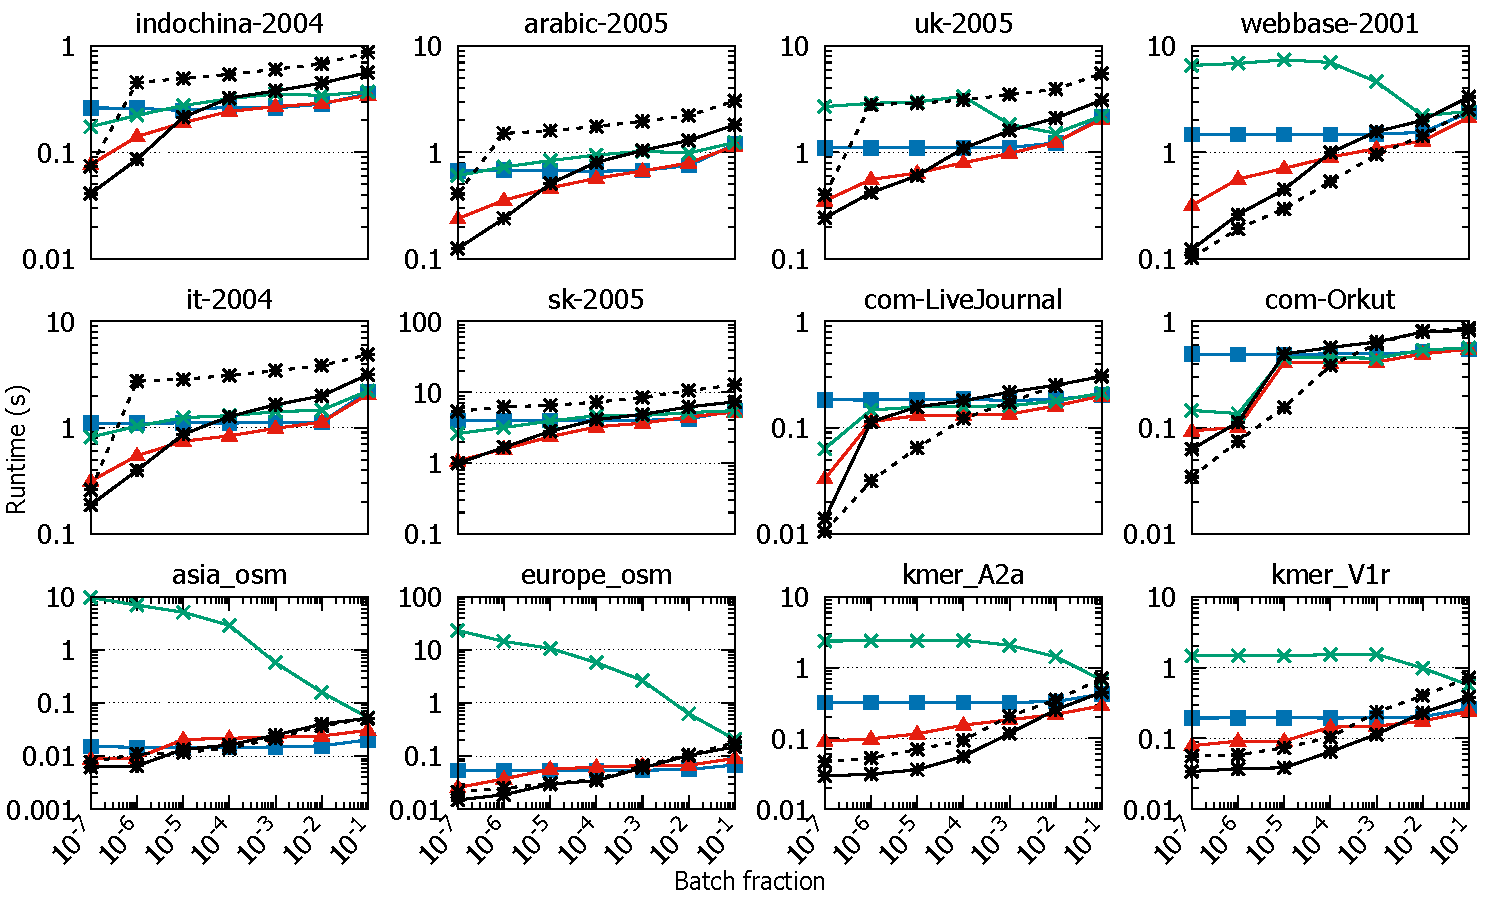
\includegraphics[width=0.58\linewidth]{out/8020-runtime-all.pdf}
  }
  \subfigure[Overall result \textbf{(CPU)}]{
    \label{fig:8020-runtime-compare--mean-cpu}
    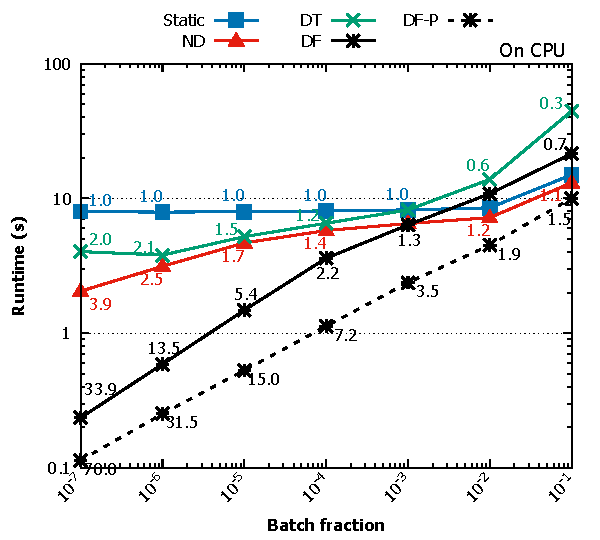
\includegraphics[width=0.38\linewidth]{out/8020-runtime-mean-cpu.pdf}
  }
  \subfigure[Results on each graph \textbf{(CPU)}]{
    \label{fig:8020-runtime-compare--all-cpu}
    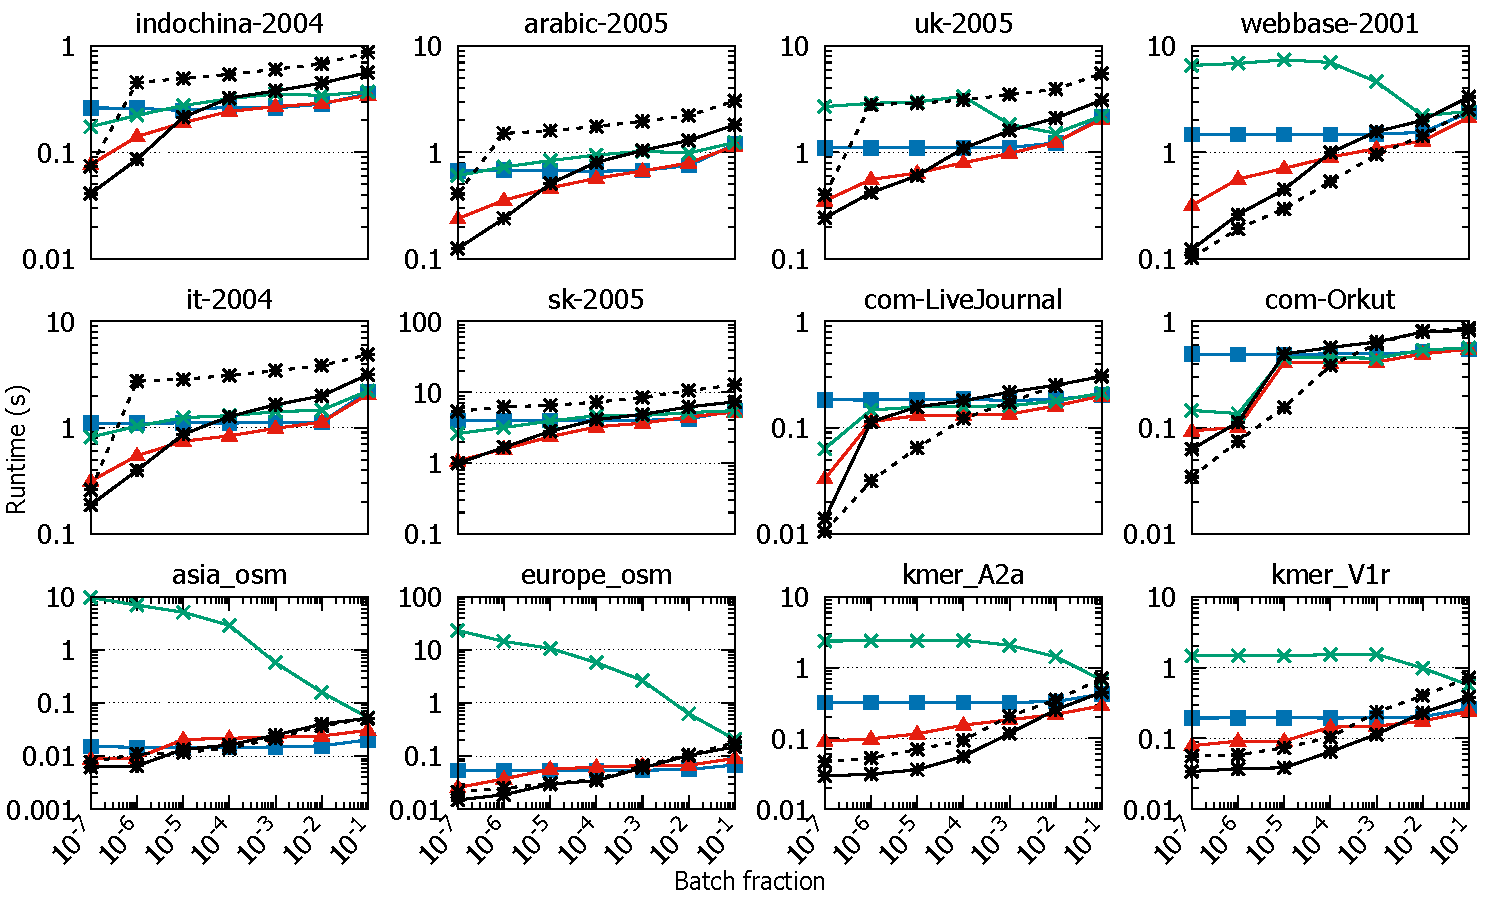
\includegraphics[width=0.58\linewidth]{out/8020-runtime-all.pdf}
  } \\[-1ex]
  \caption{Runtime (logarithmic scale) of our GPU implementation / multicore CPU implementation \cite{sahu2024df} of \textit{Static}, \textit{Naive-dynamic (ND)}, \textit{Dynamic Traversal (DT)}, \textit{Dynamic Frontier (DF)}, and \textit{Dynamic Frontier with Pruning (DF-P)} PageRank on large (static) graphs with generated random batch updates. Batch updates range in size from $10^{-7}|E|$ to $0.1|E|$ in multiples of $10$. These updates consist of $80\%$ edge insertions and $20\%$ edge deletions, mimicking realistic changes in a dynamic graph scenario. The right subfigures illustrate the runtime of each approach for individual graphs in the dataset, while the left subfigures present overall runtimes (using geometric mean for consistent scaling across graphs). Additionally, the speedup of each approach relative to Static PageRank is labeled on respective lines.}
  \label{fig:8020-runtime-compare}
\end{figure*}

\begin{figure*}[hbtp]
  \centering
  \subfigure[Overall result \textbf{(GPU)}]{
    \label{fig:8020-error-compare--mean}
    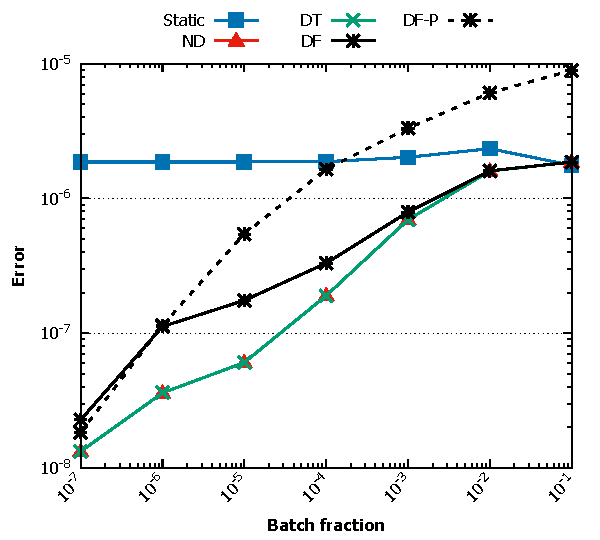
\includegraphics[width=0.38\linewidth]{out/8020-error-mean.pdf}
  }
  \subfigure[Results on each graph \textbf{(GPU)}]{
    \label{fig:8020-error-compare--all}
    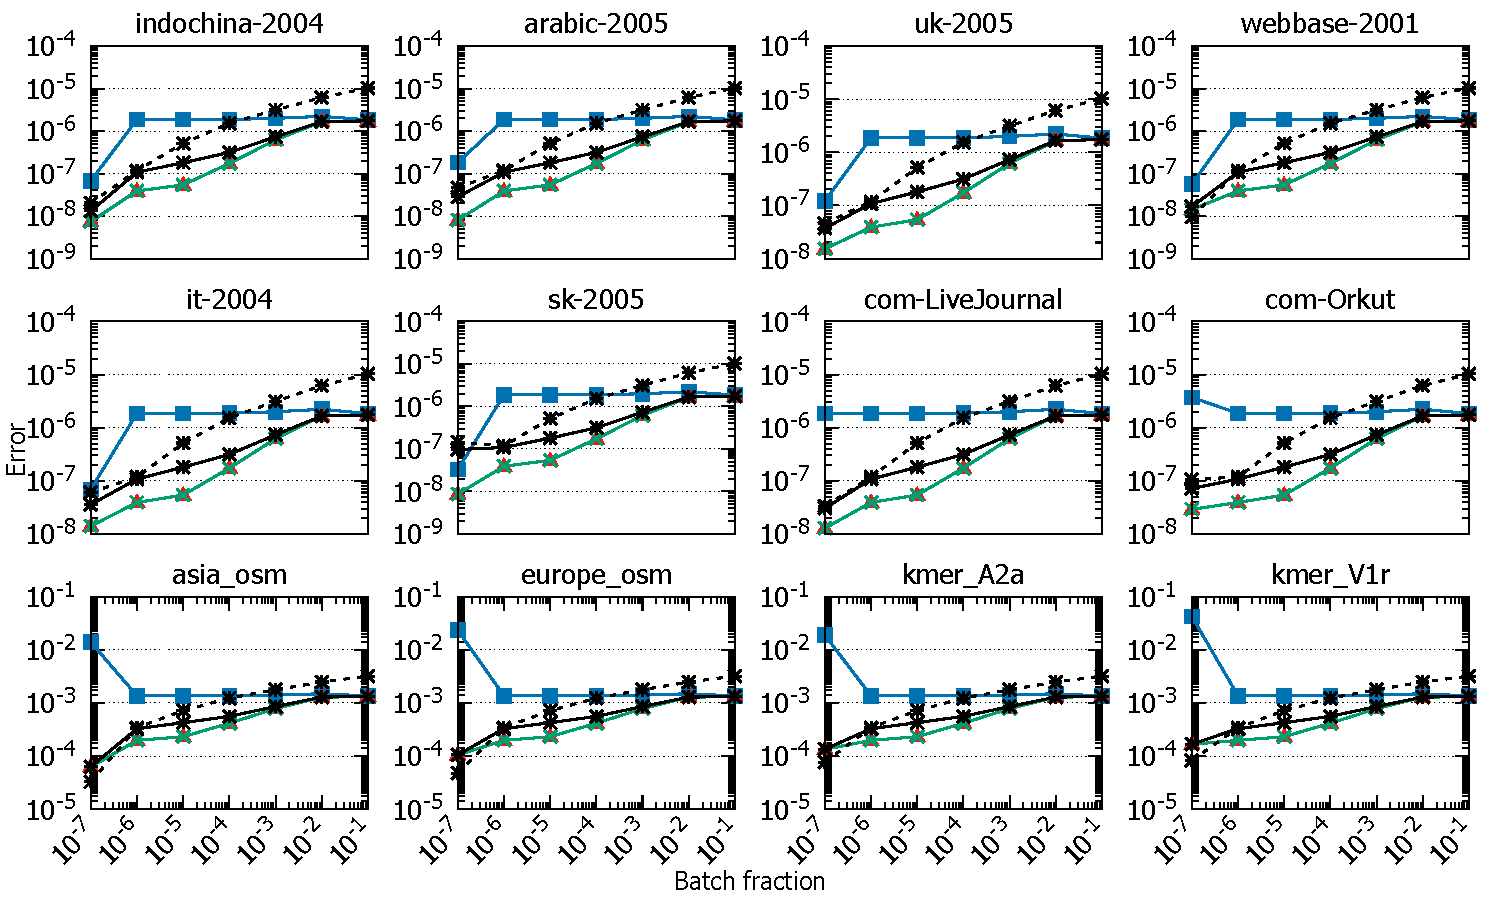
\includegraphics[width=0.58\linewidth]{out/8020-error-all.pdf}
  } \\[-1ex]
  \subfigure[Overall result \textbf{(CPU)}]{
    \label{fig:8020-error-compare--mean-cpu}
    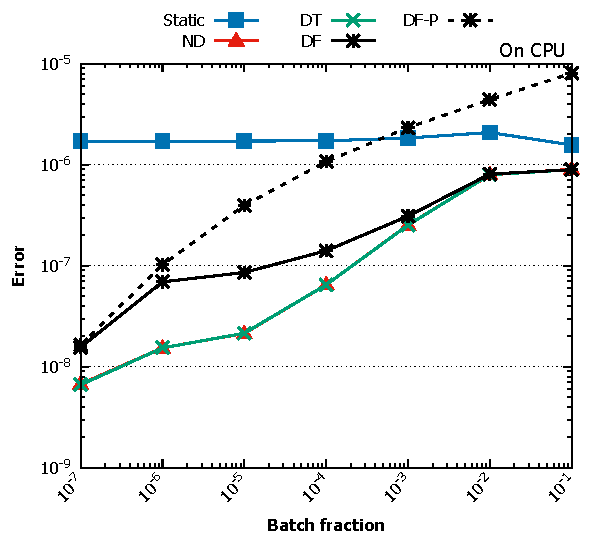
\includegraphics[width=0.38\linewidth]{out/8020-error-mean-cpu.pdf}
  }
  \subfigure[Results on each graph \textbf{(CPU)}]{
    \label{fig:8020-error-compare--all-cpu}
    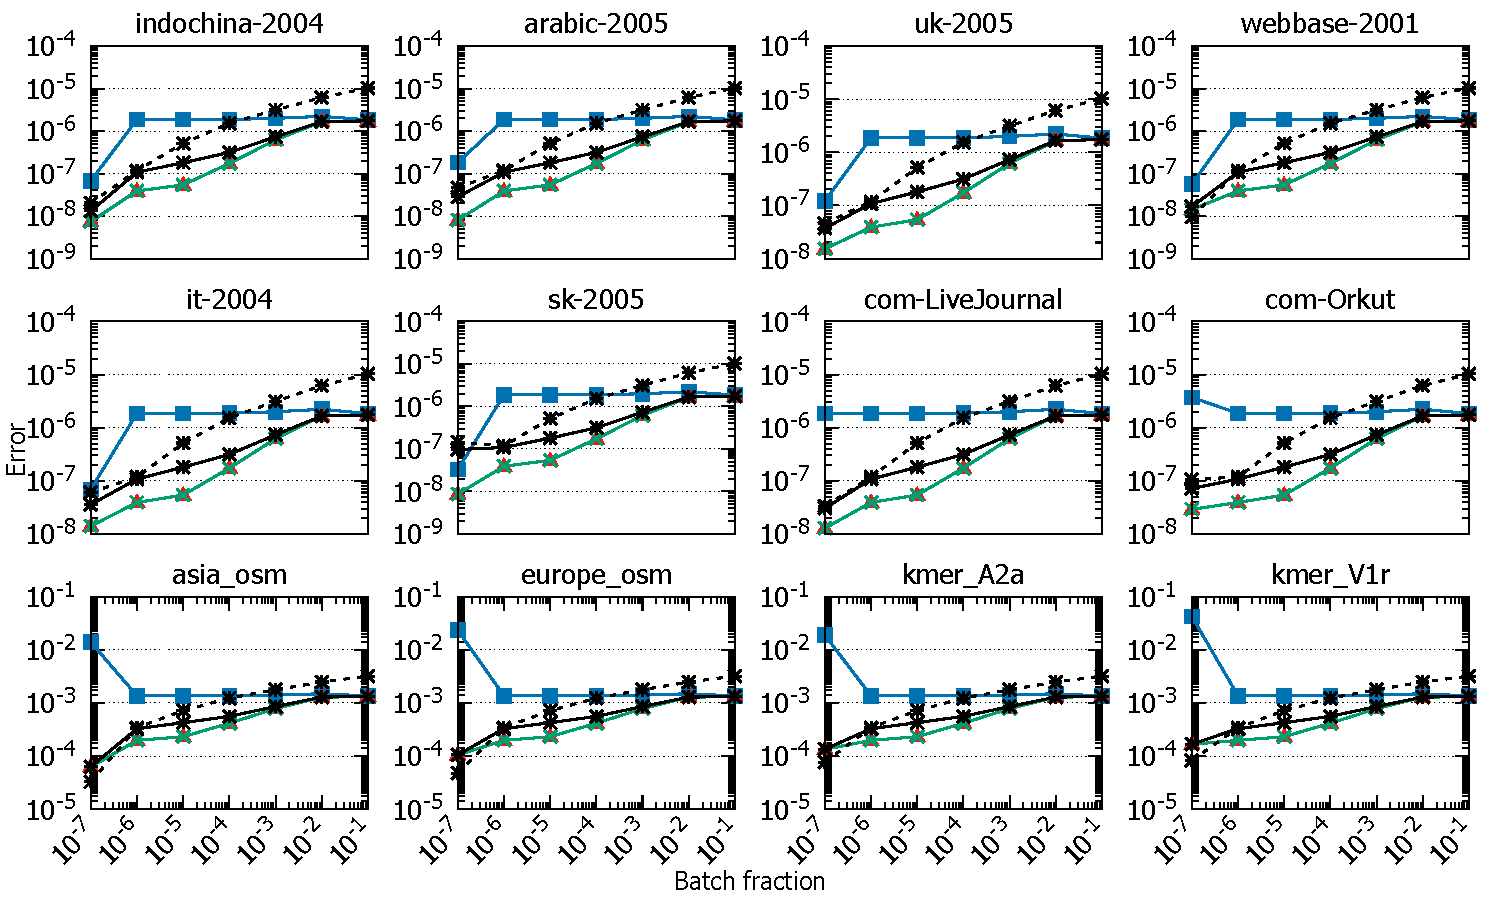
\includegraphics[width=0.58\linewidth]{out/8020-error-all.pdf}
  } \\[-1ex]
  \caption{Error comparison of \textit{Static}, \textit{Naive-dynamic (ND)}, \textit{Dynamic Traversal (DT)}, our improved \textit{Dynamic Frontier (DF)}, and \textit{Dynamic Frontier with Pruning (DF-P)} PageRank on large (static) graphs with generated random batch updates, relative to a Reference Static PageRank (see Section \ref{sec:measurement}), using $L1$-norm. The size of batch updates range from $10^{-7} |E|$ to $0.1 |E|$ in multiples of $10$ (logarithmic scale), consisting of $80\%$ edge insertions and $20\%$ edge deletions to simulate realistic dynamic graph updates. The right subfigure depicts the error for each approach in relation to each graph, while the left subfigure showcases overall errors using geometric mean for consistent scaling across graphs. \su{TODO}}
  \label{fig:8020-error-compare}
\end{figure*}


\begin{algorithm}[!hbt]
\caption{Updating ranks of vertices in parallel.}
\label{alg:update}
\begin{algorithmic}[1]
\Require{$G^t(V^t, E^t)$: Current input graph}
\Require{$R, R_{new}$: Rank vector in the previous, current iteration}
\Require{$\delta_V, \delta_N$: Is a vertex, or neighbors of a vertex affected}
\Require{$P'$: Partitioned vertex IDs --- low in-degree first }
\Require{$N'_P$: Number of vertices with low in-degree}
\Ensure{$\Delta r$: Change in rank of a vertex}
\Ensure{$\tau_f, \tau_p$: Frontier, prune tolerance}
\Ensure{$\alpha$: Damping factor}

\Statex

\Function{updateRanks}{$\delta_V, \delta_N, R_{new}, R, G^t, P', N'_P$}
  \State $\rhd$ A thread-per-vertex kernel
  \ForAll{$i \in [0, N'_P)$ \textbf{in parallel$_{thread/V}$}} \label{alg:update--thread-begin}
    \State $v \gets P'[i]$
    \If{\textbf{not} $\delta_V[v]$} \textbf{continue} \label{alg:update--affected}
    \EndIf
    \State $c \gets 0$ \textbf{;} $d \gets |G^t.out(v)|$ \label{alg:update--rank-begin}
    \State $C_0 \gets (1 - \alpha)/|V^t|$
    \ForAll{$u \in G^t.in(v)$}
      \State $c \gets c + R[u] / |G^t.out(u)|$
    \EndFor
    \If{\textbf{is \textit{DF-P}}}
      \State $r \gets 1/(1 - \alpha/d) * (C_0 + \alpha * (c - R[v]/d))$
    \Else
      \State $r \gets C_0 + \alpha * c$
    \EndIf \label{alg:update--rank-end}
    \State $\Delta r \gets |r - R[v]|$ \label{alg:update--change}
    \State $\rhd$ Prune $v$ if its relative rank change is small
    \If{\textbf{is \textit{DF-P} and} $\Delta r / \max(r, R[v]) \leq \tau_p$} \label{alg:update--prune-begin}
      \State $\delta_V[v] \gets 0$
    \EndIf \label{alg:update--prune-end}
    \State $\rhd$ Expand frontier if relative rank change is large
    \If{$\Delta r / \max(r, R[v]) > \tau_f$} \label{alg:update--expand-begin}
      \State $\delta_N[v] \gets 0$
    \EndIf \label{alg:update--expand-end}
    \State $\rhd$ Update rank of $v$
    \State $R[v] \gets r$ \label{alg:update--update}
  \EndFor \label{alg:update--thread-end}
  \State $\rhd$ Similarly with block-per-vertex kernel
  \State $\rhd$ (using block-reduce, requires shared memory)
  \ForAll{$i \in [N'_P, |V^t|)$ \textbf{in parallel$_{block/V}$}} \label{alg:update--block-begin}
    \State $\cdots$
  \EndFor \label{alg:update--block-end}
\EndFunction
\end{algorithmic}
\end{algorithm}

\begin{algorithm}[!hbt]
\caption{Parallel vertex partitioning by degree.}
\label{alg:partition}
\begin{algorithmic}[1]
\Require{$G(V, E)$: Input graph}
\Ensure{$D_P$: Maximum degree of a low-degree vertex}
\Ensure{$B_k$: Temporary buffer used for partitioning}
\Ensure{$P$: Partitioned vertex IDs --- low degree vertices first }
\Ensure{$N_P$: Number of vertices with low degree}

\Statex

\Function{partition}{$G$}
  \State $P \gets B_k \gets \{\}$ \label{alg:partition--initialize}
  \State $\rhd$ Populate vertex IDs with degree $\leq D_P$
  \ForAll{$v \in V$ \textbf{in parallel}} \label{alg:partition--less-begin}
    \State $B_k[v] \gets |G.out(v)| \leq D_P$
  \EndFor \label{alg:partition--less-end}
  \State $B_k[|V|] \gets 0$ \label{alg:partition--lscan-begin}
  \State $exclusiveScan(B_k)$ \textbf{;} $N_P \gets B_k[|V|]$ \label{alg:partition--lscan-end}
  \ForAll{$v \in V$ \textbf{in parallel}} \label{alg:partition--lpopulate-begin}
    \If{$|G.out(v)| \leq D_P$} $P[B_k[v]] \gets v$
    \EndIf
  \EndFor \label{alg:partition--lpopulate-end}
  \State $\rhd$ Populate vertex IDs with degree $> D_P$
  \ForAll{$v \in V$ \textbf{in parallel}} \label{alg:partition--greater-begin}
    \State $B_k[v] \gets |G.out(v)| > D_P$
  \EndFor \label{alg:partition--greater-end}
  \State $exclusiveScan(B_k)$ \label{alg:partition--gscan}
  \ForAll{$v \in V$ \textbf{in parallel}} \label{alg:partition--gpopulate-begin}
    \If{$|G.out(v)| > D_P$} $P[N_P + B_k[v]] \gets v$
    \EndIf
  \EndFor \label{alg:partition--gpopulate-end}
  \State \ReturnInline{$\{P, N_P\}$} \label{alg:partition--return}
\EndFunction
\end{algorithmic}
\end{algorithm}

\begin{algorithm}[!hbt]
\caption{Parallel marking of affected vertices.}
\label{alg:affected}
\begin{algorithmic}[1]
\Require{$G^t(V^t, E^t)$: Current input graph}
\Require{$\Delta^{t-}, \Delta^{t+}$: Edge deletions and insertions (input)}
\Require{$\delta_V, \delta_N$: Is a vertex, or neighbors of a vertex affected}
\Require{$P$: Partitioned vertex IDs (low-degree vertices first) }
\Require{$N_P$: Number of vertices with low degree}

\Statex

\Function{initialAffected}{$G^t, \Delta^{t-}, \Delta^{t+}$}
  \State $N_D \gets |\Delta^{t-}|$ \textbf{;} $N_I \gets |\Delta^{t+}|$ \label{alg:affected--iinitialize}
  \State $\rhd$ For edge deletions
  \ForAll{$i \in [0, N_D)$ \textbf{in parallel}} \label{alg:affected--idel-begin}
    \State $u \gets \Delta^{t-}[i].source$
    \State $v \gets \Delta^{t-}[i].target$
    \State $\delta_N[u] \gets 1$
    \State $\delta_V[v] \gets 1$
  \EndFor \label{alg:affected--idel-end}
  \State $\rhd$ For edge insertions
  \ForAll{$i \in [0, N_I)$ \textbf{in parallel}} \label{alg:affected--iins-begin}
    \State $u \gets \Delta^{t+}[i].source$
    \State $\delta_N[u] \gets 1$
  \EndFor \label{alg:affected--iins-end}
  \Return{$\{\delta_V, \delta_N\}$} \label{alg:affected--ireturn}
\EndFunction

\Statex

\Function{expandAffected}{$\delta_V, \delta_N, G^t, P, N_P$}
  \State $\rhd$ A thread-per-vertex kernel
  \ForAll{$i \in [0, N_P)$ \textbf{in parallel$_{thread/V}$}} \label{alg:affected--ethread-begin}
    \State $u \gets P[i]$
    \If{$\delta_N[u]$} $markNeighbors(\delta_V, G^t, u)$ \label{alg:affected--etmark}
    \EndIf
  \EndFor \label{alg:affected--ethread-end}
  \State $\rhd$ Similarly with block-per-vertex kernel
  \ForAll{$i \in [N_P, |V^t|)$ \textbf{in parallel$_{block/V}$}} \label{alg:affected--eblock-begin}
    \State $\cdots$
  \EndFor \label{alg:affected--eblock-end}
\EndFunction
\end{algorithmic}
\end{algorithm}





\subsection{Indirect Comparison with State-of-the-art PageRank Implementations (Static)}
\label{sec:static-comparison-indirect}

We now indirectly compare the performance of our GPU implementation of Static PageRank with other similar state-of-the-art implementations. Chen et al. \cite{chen2022atos} present Atos, a state-of-the-art task-parallel GPU scheduler for graph analytics. They say that in Gunrock and other frameworks, each frontier in a graph sweep is launched as a separate GPU kernel in the BSP model. This may result in insufficient parallelism, uneven finish times, and high kernel launch overhead for small frontiers. In contrast, Chen et al. present a persistent task scheduler which runs continuously to minimize kernel launch overhead, and also support asynchronous execution. For PageRank, they present a push-based asynchronous PageRank (requires many atomic ops) that uses a frontier to keep track of vertices that need to be processed in the next iteration. They use a queue to keep track fo the frontier (also requires atomic ops). Their CUDA kernel appears to be barrier-free. Their frontier concept is similar to ours \cite{sahu2024df}, but they do not use it for Dynamic PageRank. Chen et al. are able to achieve $3.2\times$ speedup over Gunrock on the \textit{indochina-2004} graph (see Table $1$ of their paper \cite{chen2022atos}). However, on the same graph, we achieve $24.4\times$ speedup over Gunrock (see Figure \ref{fig:compare--speedup} in this report).

In another work, Chen et al. \cite{chen2022scalable} extend their Atos dynamic scheduling framework to multi-node GPU systems that supports Partitioned Global Address Space (PGAS) style lightweight one-sided memory operations within and between nodes. However on the \textit{indochina-2004} graph, even with $4$ GPUs, they are unable to beat our speedup with respect to Gunrock (see Table $4$ of their paper \cite{chen2022scalable}, and Figure \ref{fig:compare--speedup} in this report).

Yang et al. \cite{yang2022graphblast} present GraphBLAST, A High-Performance Linear Algebra-based Graph Framework on the GPU. They discuss that GraphBLAS has lacked high-performance implementations for GPUs. Further, they say that GraphBLAS Template Library (GBTL), a GraphBLAS-inspired GPU graph framework, is an order of magnitude slower than state-of-the-art graph frameworks on the GPU in terms of performance. They say, the issue lies with the lack of generalizability of optimizations, irregular memory access patterns and load imbalance, and low compute-to-memory access ratio. Their new design principles include exploiting input sparsity, which allows users to write graph algorithms without specifying push and pull direction, exploiting output sparsity allows users to tell the backend which values of the output in a single vectorized computation they do not want computed, and load-balancing. For SpMV load balancing (like PageRank) they discuss two main approaches, row split, which seems like block-per-vertex; and merge-based, which seems like edge balanced between threads/blocks. For PageRank, they use merge-based load balancing with segmented scan. They also use a heuristic to switch between push- and pull-based approach. They say that the optimal time to switch from push to pull is very early on (as Ligra). On the \textit{indochina-2004} graph, they are able to achieve $2.2\times$/$1.2\times$ speedup over Gunrock (see Table $12$/$13$ in their paper \cite{yang2022graphblast}). However, on the same graph, we achieve $24.4\times$ speedup over Gunrock (see Figure \ref{fig:compare--speedup} in this report).

Wang et al. \cite{wang2021grus} present Grus, a Unified-memory-efficient High-performance Graph Processing on GPU. They focus on addressing the following, related to Unified Memory (UM): minimizing the amount of migrated data; reducing the number of page faults; and reducing page migration overhead. They achieve this with their framework with memory management and execution optimization. They use CSR as a space-efficient data structure for graph representation, and use $5|V|$ bytes for representing a frontier. They use an adaptive UM policy, where the frontier and ranks are assigned high priority, the CSR index array is assigned medium priority, and the CSR edges array is assigned low priority. They also use a Bitmap-directed frontier (8-bit integer array, similar to ours, plus a queue - no atomic ops needed), and use warp-centric load balancing (warp-per-vertex, similar to block-per-vertex, no partitioning) for PageRank computation. On the \textit{uk-2005} graph, they are able to achieve a $1.2\times$ speedup over Gunrock (see Table $4$ in their paper \cite{wang2021grus}). However, we get $8.6\times$ speedup over Gunrock on the same graph (see Figure \ref{fig:compare--speedup} in this report).

Concessao et al. \cite{concessao2023meerkat} propose a library-based framework for dynamic graph algorithms that utilizes a GPU-tailored graph representation and exploits the warp-cooperative execution model. The library, named Meerkat, builds upon a recently proposed dynamic graph representation on GPUs. This representation exploits a hashtable-based mechanism to store a vertex’s neighborhood. Meerkat also enables fast iteration through a group of vertices, such as the whole set of vertices or the neighbors of a vertex. They find that these two iteration patterns are common, and optimizing them is crucial for achieving performance. Meerkat supports dynamic edge additions and edge deletions, along with their batched versions. The PageRank implementation of Meerkat performs, on average, $1.7\times$ faster than Hornet. However, our Static PageRank is on average $31\times$ faster than Hornet (see Figure \ref{fig:compare--speedup} in our report).
